\documentclass[12pt,a4paper,cours,firamath]{nsi}
\begin{document}

% \begin{titlepage}
    \begin{center}
        
\includegraphics[width=12cm]{titlepage/img/yin_yang_python}\\[2em]

        {\bigtitlefont \large\color{gray} Programmation avec Python}

        {\titlefont\Large\color{gray} Spécialité numérique et sciences informatiques en classe de première\\[2em]}

        {\color{gray}\textbf{Lycée Rabelais\\ Saint Brieuc\\ 2023-2024}}
    \end{center}
\end{titlepage}

%  \part{Programmation avec Python}

% \chapter{Valeurs et types}
\label{ch:valeurs}
\section{Python, machine à évaluer}
\textsc{Python} est en premier lieu une machine à calculer, ou plutôt une machine à \textit{évaluer} : lorsque \textsc{Python} rencontre une \textit{expression}, c'est-à-dire une écriture qui produit une valeur, il commence par déterminer cette valeur.\\
Pour s'en rendre compte, il suffit d'écrire des expressions dans une \textit{console}.
\begin{pyc}
  \begin{minted}{python}
        >>> 5 - 3
        2
        
        >>> 11 / (1 + 2)
        3.6666666666666665

        >>> 30 / 15
        2.0
    \end{minted}
\end{pyc}
On se rend compte que les valeurs rencontrées ne sont pas présentées de la même manière :\\ \mintinline{python}{5 - 3} a la valeur \mintinline{python}{2} alors que \mintinline{python}{30 / 15} a la valeur \mintinline{python}{2.0}.\\
Pour y voir plus clair, on peut appeler la fonction \mintinline{python}{type} qui
\begin{itemize}
  \item en entrée prend une expression ;
  \item renvoie le \textit{type} de l'expression.
\end{itemize}
\begin{pyc}
  \begin{minted}{python}
    >>> type(2)
    <class int>

    >>> type(2.0)
    <class float>
  \end{minted}
\end{pyc}

Il y a donc au moins deux types de valeurs, le type \mintinline{python}{int} et le type \mintinline{python}{float}.\\
En fait il existe une multitude de types prédéfinis selon la nature de la valeur à représenter et nous allons les passer en revue.


\section{Le type int}
\label{sec:int}
Il sert à représenter les \textit{entiers relatifs} (\textit{integer} signifie  « entier » en Anglais).\\
Le type \mintinline{python}{int} dispose des opérations \mintinline{python}{+} (addition), \mintinline{python}{-} (soustraction) et \mintinline{python}{*} (multiplication).

\begin{pyc}\begin{minted}{python}
>>> 3 + 2
5

>>> 2 * 3
6

>>> 3 - 2 * 2
-1

>>> 10_000 # on utilise des _ pour séparer les chiffres
\end{minted}
\end{pyc}

Les parenthèses sont utilisées comme en mathématiques, pour indiquer une \textit{priorité opératoire}. Cependant les crochets et les accolades sont réservés à un autre usage.

\begin{pyc}
  \begin{minted}{python}
    >>> (3 + 4) * 5
    35
  \end{minted}
\end{pyc}

On dispose également de \textit{deux opérations très pratiques} : soient \mintinline{python}{a} et \mintinline{python}{b} deux \mintinline{python}{int}, et \mintinline{python}{b} non nul, alors on
\begin{itemize}
  \item \mintinline{python}{a // b} est le \textit{quotient} de la \textit{division euclidienne} de \mintinline{python}{a} par \mintinline{python}{b} ;
  \item \mintinline{python}|a % b| est le \textit{reste}.
\end{itemize}


\begin{pyc}\begin{minted}{python}
>>> 64 // 10 # 64, c'est 6 * 10 + 4
6

>>> 64 % 10
4

>>> 22 // 7 # 22, c'est 3 * 7 + 1
3

>>> 22 % 7
1
\end{minted}
\end{pyc}


On dispose de l'opération d'\textit{exponentiation} (opération puissance), notée \mintinline{python}{**}.\\
\textbf{Attention :} Cette opération peut produire un résultat \textit{non-entier}, de type \mintinline{python}{float} (voir partie suivante).

\begin{pyc}\begin{minted}{python}
>>> 2 ** 3
8

>>> 10 ** 4
10000

>>> 2 ** (-1)
0.5
\end{minted}
\end{pyc}

Pour finir, la \textit{division décimale} peut être effectuée sur des entiers, mais elle renvoie un résultat de type \mintinline{python}{float}.

\section{Le type float}
Il sert à représenter les \textit{nombres à virgule flottante} (\textit{to float} : flotter en Anglais). Ce sont (en gros) des nombres
décimaux.\ \textsc{Python} comprend et utilise la notation scientifique : \mintinline{python}{2.35e6} vaut $2,35\times 10^6$, c'est-à-dire 2 350 000.

\begin{pyc}\begin{minted}{python}
>>>  2 / 7
0.2857142857142857 # c'est une valeur approchée

>>> 1 / 100_000
1e-05

>>> 1.2e-4
0.00012
\end{minted}
\end{pyc}

On peut pratiquer sur les \mintinline{python}{float} toutes les opérations vues avec les \mintinline{python}{int}. Pour des fonctions plus compliquées telles le cosinus ou
l'exponentielle, on fait appel au module\footnote{Un module est un ensemble de \textit{fonctions} et/ou de \textit{constantes} que l'on peut importer.}
\mintinline{python}{math} :

\begin{pyc}\begin{minted}{python}
>>> from math import *
>>> pi
3.141592653589793

>>> cos(pi / 3)
0.5000000000000001

>>> exp(2)
7.38905609893065

>>> log(2)
0.6931471805599453

>>> exp(log(2))
2.0
\end{minted}
\end{pyc}

\mintinline{python}{exp} est la \textit{fonction exponentielle} et \mintinline{python}{log} la \textit{fonction logarithme népérien}\footnote{Voir le programme de mathématiques
  de terminale scientifique.} notée $\ln$ en France.



\section{Le type str}

Il sert à représenter les \textit{chaînes de caractères} (\mintinline{python}{str} est l'abréviation de \textit{string}, qui veut dire chaîne en anglais).
Lorsqu'on écrit une valeur de type \mintinline{python}{str}, on peut utiliser les symboles \mintinline{python}{'}, \mintinline{python}{"} ou même \mintinline{python}{'''} (suivant que la chaîne contient des apostrophes, ou des guillemets).

\begin{pyc}\begin{minted}{python}
>>> 'Bonjour.'
'Bonjour'

>>> 'J'aime Python.'
SyntaxError

>>> "J'aime Python."
"J'aime Python."

>>> "Je n'aime pas qu'on m'appelle "geek"."
SyntaxError

>>> """Je n'aime pas qu'on m'appelle "geek"."""
'Je n\'aime pas qu\'on m\'appelle "geek".'
\end{minted}
\end{pyc}
La dernière évaluation produit une valeur correcte. \textsc{Python} utilise simplement \mintinline{python}{\'} pour écrire les apostrophes qui sont à l'intérieur de la valeur.\\


Le symbole \mintinline{python}{+} sert à \textit{concaténer 2 chaînes}, c'est-à-dire à les mettre bout à bout.

\begin{pyc}\begin{minted}{python}
>>> 'Yes' + 'No'
'YesNo'

>>> 'No' + 'Yes'
'NoYes'
\end{minted}
\end{pyc}

On peut même multiplier un \mintinline{python}{str} par un \mintinline{python}{int} :
\begin{pyc}
  \begin{minted}{python}
    >>> 3 * 'Aïe ! '
    'Aïe ! Aïe ! Aïe ! '
  \end{minted}
\end{pyc}
\textsc{Python} évalue \mintinline{python}{3*'Aïe !'} comme \mintinline{python}{'Aïe ! ' + 'Aïe ! ' + 'Aïe ! '}.


Voici deux types très utiles que nous étudierons en détail plus tard.

\section{Le type list}

Une valeur de type \mintinline{python}{list} est une... liste ordonnée de valeurs. Celles-ci peuvent être du même type ou non.

\begin{pyc}
  \begin{minted}{python}
    >>> [] # liste vide
    []

    >>> [1, 4, 5] # liste comportant 3 int
    [1, 4, 5]

    >>> [2.0, -4, 'Bonjour', 'Coucou']
    [2.0, -4, 'Bonjour', 'Coucou']
  \end{minted}
\end{pyc}

L'intérêt de ce type est de rassembler plusieurs valeurs au sein d'une seule, qui pourra ensuite être \textit{parcourue}.

\section{Le type dict}

Celui-ci sert à établir des \textit{associations} du type \textit{clé : valeur}.

\begin{pyc}
  \begin{minted}{python}
      >>> {} # dictionnaire vide
      {}

      >>> {'France': 'Paris', 'Canada': 'Ottawa', 'Pays-Bas': 'La Haye'}
      {'France': 'Paris', 'Canada': 'Ottawa', 'Pays-Bas': 'La Haye'}
    \end{minted}
\end{pyc}

Tout comme le type \mintinline{python}{list}, ce type sert à \textit{structurer les données}. L'exemple précédent fait correspondre des capitales à des pays.



\section{Le type bool}
Il sert à représenter les \textit{valeurs booléennes}, valant \mintinline{python}{True} (vrai) ou
\mintinline{python}{False} (faux).

\begin{pyc}\begin{minted}{python}
>>> False
False

>>> True
True
\end{minted}
\end{pyc}

Cela peut paraître un peu pauvre, c'est trompeur : les \textit{expressions logiques} sont des écritures dont la valeur est un booléen. Lorsque \textsc{Python} les rencontre, il les évalue pour trouver soit \mintinline{python}{True} soit \mintinline{python}{False}.

\begin{pyc}
  \begin{minted}{python}
    >>> 3 >= 2 # évalue si 3 est supérieur ou égal à 2
    True
    
    >>> 3 + 5 == 2 # évalue si 3 + 5 vaut 2
    False

    >>> 1 in [3, 4, 1, 5] # évalue si 1 est un élément de la liste
    True
  \end{minted}
\end{pyc}

\begin{encadrecolore}{Attention}{UGLiRed}
  Pour \textit{tester} si deux valeurs sont égales, on utilise \mintinline{python}{==}  (et pas \mintinline{python}{=} ).

\end{encadrecolore}


Ce type dispose d'\textit{opérations logiques} : \mintinline{python}{or} (ou), \mintinline{python}{and} (et) et \mintinline{python}{not} (non).

\begin{pyc}\begin{minted}{python}
>>> True and False # vrai que si les 2 sont vrais
False

>>> True or False # faux que si les 2 sont faux
True

>>> not (3 < 1) # contraire
True

>>> (2 < 1) or (3 >= 0)
True
\end{minted}
\end{pyc}
% \chapter{Variables et affectations}

\section{Le symbole =}

En mathématiques, le symbole $=$ a plusieurs significations
\begin{itemize}
	\item dans $2+2=4$, on peut comprendre $=$ comme un opérateur d'évaluation : $2+2$, cela « donne » $4$ ;
	\item dans $\mathcal{P}=2\times(\ell+L)$, on peut considérer que $=$ sert à définir ce qu'est le périmètre d'un rectangle de dimensions $\ell$ et $L$ ;
	\item dans $3x + 2 = 4x +5$, le $=$ sert à convenir que les 2 membres ont la même valeur et on cherche s'il existe un ou des nombres $x$ qui satisfont l'égalité (appelée équation) ;
	\item \textit{et cætera}.
\end{itemize}

En \textsc{Python}, le symbole \mintinline{python}{=}  n'a qu'un seul sens : il sert à l'\textit{affectation}.

\section{L'affectation}
Il s'agit de « stocker » une valeur dans un endroit de la mémoire auquel \textsc{Python} donne un nom\footnote{En réalité c'est plus compliqué mais cela ne nous intéresse pas.}. Voici un exemple d'affectation :
\begin{center}\Large
	\mintinline{python}{a = 2}
\end{center}\
\begin{itemize}
	\item   \mintinline{python}{2} est une \textit{valeur} de type \mintinline{python}{int} ;
	\item   la \textit{variable} \mintinline{python}{a} est créée ;\
	\item   \mintinline{python}{a} est « attachée » à la valeur \mintinline{python}{2} ;
	\item   par extension \mintinline{python}{a} est également de type \mintinline{python}{int}.
\end{itemize}
Au cours d'un programme la valeur associée à une variable peut change\ldots D'où le nom de \textit{variable}.\\


\begin{definition}[ : affectation]
	Lors d'une affectation
	\begin{itemize}
		\item d'abord \textsc{Python} évalue ce qu'il y a à droite du symbole \mintinline{python}{=} ;
		\item ensuite il affecte cette valeur à la variable qui figure à gauche du symbole \mintinline{python}{=} ;
		\item si la variable n'existe pas déjà, elle est créée automatiquement ;
		\item le type de la variable, c'est le type de la valeur qu'on lui affecte.
	\end{itemize}
\end{definition}
Que fait le programme suivant ?

\begin{pyc}
	\begin{minted}{python}
x = 0
x = x + 1
print(x)    
\end{minted}
\end{pyc}

\begin{itemize}
	\item il crée une variable \mintinline{python}{x} de type \mintinline{python}{int} valant \mintinline{python}{0} ;
	\item il évalue \mintinline{python}{x + 1}, trouve \mintinline{python}{1} et affecte cette valeur à \mintinline{python}{x} ;
	\item évalue \mintinline{python}{x}, trouve 1 et donc affiche \mintinline{python}{1}.
\end{itemize}

\begin{aretenir}
	En mathématiques, $x = x + 1$ est une équation sans solution.\\

	En \textsc{Python}, l'instruction \mintinline{python}{x = x + 1} sert à augmenter la valeur de \mintinline{python}{x} de 1 (on dit aussi \textit{incrémenter}).
\end{aretenir}

\subsection{Affectations multiples}
\textsc{Python} permet d'affecter plusieurs valeurs à plusieurs variables en même temps.

\begin{pyc}\begin{minted}{python}
>>> a, b = 10, 2
>>> a
10

>>> b
2

>>> a, b = b, a # permet d'échanger a et b
>>> a
2

>>> b
10

\end{minted}
\end{pyc}

\subsection{Notation condensée}
On est souvent amené à écrire des instructions telles que  \mintinline{python}{a = a + 1} ou \mintinline{python}{b = b / 2}. Cela peut être lourd quand les variables ne s'appellent
pas \mintinline{python}{a} ou \mintinline{python}{b} mais \mintinline{python}{rayon_sphere} ou \mintinline{python}{largeur_niveau}. On peut utiliser les notation suivantes :
\begin{pyc}\begin{minted}{python}
>>> rayon_sphere = 3.4
>>> rayon_sphere /= 2
>>> rayon_sphere
1.7

>>> largeur_niveau = 19
>>> largeur_niveau += 1
>>> largeur_niveau
20
\end{minted}
\end{pyc}

On dispose également de \mintinline{python}{*=}, \mintinline{python}{//=}, \mintinline{python}|%=|, \mintinline{python}{-=} et \mintinline{python}{**=}.

\section{Le cas des variables de type str ou list}

\subsection{Les str}

Les valeurs de type \mintinline{python}{str} sont composées de caractères \emph{alphanumériques}. On peut accéder à chacun d'eux de la manière suivante :
\begin{pyc}\begin{minted}{python}
>>> chaine = 'Bonjour !'
>>> chaine[0]
'B'
>>> chaine[5]
'u'
\end{minted}
\end{pyc}

Voici comment \textsc{Python} représente  la chaîne précédente :

\begin{center}
	\alternaterowcolors
	\tabstyled
	\begin{tabular}{|c|c|c|c|c|c|c|c|c|c|}
		\hline
		\ccell i    & \ccell 0 & \ccell 1 & \ccell 2 & \ccell 3 & \ccell 4 & \ccell 5 & \ccell 6 & \ccell 7 & \ccell 8 \\
		\hline
		\mintinline{python}{chaine[i]} & B      & o      & n      & j      & o      & u      & r      &        & !      \\
		\hline
	\end{tabular}
\end{center}

On a parfois besoin de connaître la longueur (\emph{length} en anglais) d'une chaîne de caractères :

\begin{pyc}\begin{minted}{python}
>>> chaine = 'onzelettres'
>>> len(chaine)
11
\end{minted}
\end{pyc}

On peut aussi accéder facilement au dernier (ou à l'avant dernier) caractère d'une variable de type \mintinline{python}{str} :

\begin{pyc}
	\begin{minted}{python}
>>> a = "M'enfin ?!"
>>> a[-1]
'!'

>>> a[-2]
'?'
\end{minted}
\end{pyc}

\subsection{Les list}

Cela se passe un peu comme pour les \mintinline{python}{str}

\begin{pyc}
	\begin{minted}{python}
		>>> lst = [3, 4, 8]
		>>> lst[1] # élément d'indice 1 de lst
		4

		>>> lst[-1] # dernier élément de lst
		8

		>>> len(lst)
		3
	\end{minted}
\end{pyc}

Lorsqu'on essaie d'accéder à un élément dont l'indice est supérieur ou égal à la longueur de la liste, on obtient une erreur. Dans l'exemple précédent si on évalue \mintinline{python}{lst[3]} on obtient :
\color{UGLiRed}
\begin{verbatim}
IndexError: list index out of range	
\end{verbatim}
\color{black}

Une étude détaillée des \mintinline{python}{list} est faite au chapitre \ref{ch:listes}.


% \chapter{Entrées-sorties et transtypage}

\section{Entrées-sorties}

Lorsqu'on écrit un programme en \textsc{Python}, on a très souvent besoin
\begin{itemize}
    \item qu'il affiche des informations à l'écran ;
    \item qu'il demande des informations à l'utilisateur\cdot trice.
\end{itemize}

\subsection{la fonction print}

C'est elle qui sert à afficher à l'écran :

\begin{pyc}
    \begin{minted}{python}
        print("Bonjour") # affiche bonjour
        print(4) # affiche 4
        print(2 + 4) # évalue 2 + 4 et affiche 6
        a = 3
        print(a) évalue a et affiche 3
    \end{minted}
\end{pyc}

On peut s'en servir de diverses manières :
\begin{pyc}
    \begin{minted}{python}
        age = 16
        print("Vous avez", age, "ans.")
    \end{minted}
\end{pyc}
Dans ce premier cas, on a donné 3 paramètres à \mintinline{python}{print}:
\begin{itemize}
    \item le \mintinline{python}{str "Vous avez"} ;
    \item la variable \mintinline{python}{age} ;
    \item  le \mintinline{python}{str "ans."}.
\end{itemize}
On peut aussi utiliser ce qu'on appelle une « f-string » de la manière suivante :
\begin{pyc}
    \begin{minted}{python}
        age = 16
        print(f"Vous avez {age} ans.") # noter le f au début
    \end{minted}
\end{pyc}
Dans ce cas, \textsc{Python} construit le \mintinline{python}{str} à afficher en y reportant la valeur de \mintinline{python}{age}.\\
C'est cette méthode que nous utiliserons par la suite.\\

Enfin, \mintinline{python}{print} revient à la ligne par défaut, mais on peut changer cela :
\begin{pyc}
    \begin{minted}{python}
        print("Bonjour",end="") # aucun retour à la ligne
        print("à tous",end="!") # aucun retour et ! à la fin
    \end{minted}
\end{pyc}
Ce programme affiche \texttt{Bonjour à tous!} sans revenir à la ligne.

\subsection{La fonction input}
C'est elle qui est chargée de récupérer des informations que l'utilisateur\cdot trice entre au clavier.
\begin{pyc}
    \begin{minted}{python}
        nom = input("Entrez votre nom : ")
    \end{minted}
\end{pyc}
Le programme précédent
\begin{itemize}
    \item affiche \mintinline{python}{Entrez votre nom : } ;
    \item attend que l'utilisateur\cdot trice tape quelque chose, puis valide avec la touche d'entrée ;
    \item stocke le message tapé dans la variable \mintinline{python}{nom}.
\end{itemize}
\begin{encadrecolore}{Important}{UGLiRed}
    La valeur renvoyée par la fonction \mintinline{python}{input} est \textit{toujours} de type \mintinline{python}{str}. Cela va donc nous amener à faire du \textit{transtypage}.
\end{encadrecolore}

\section{Transtypage}

\begin{definition}[ : transtypage]
    C'est l'action de changer le type d'une valeur ou d'une variable en un autre type \textit{compatible}.
\end{definition}

Voici un exemple :
\begin{pyc}
    \begin{minted}{python}
        a = 2 # a est un int
        b = float(a) # la valeur 2 est convertie en float et stockée dans b
        print(b) # affiche 2.0
    \end{minted}
\end{pyc}

En voici un autre dont nous nous servirons beaucoup
\begin{pyc}
    \begin{minted}{python}
        a = '12' # a est un str
        b = int(a) # '12' est converti en l'entier 12
        print(b + 1) # évalue b + 1 à 13 et affiche 13
    \end{minted}
\end{pyc}

\begin{encadrecolore}{Attention}{UGLiRed}
    Le transtypage n'est pas une action anodine et peut produire des erreurs lorsque la valeur à transtyper est incompatible avec le nouveau type qu'on veut lui donner.
\end{encadrecolore}

\begin{pyc}
    \begin{minted}{python}
        a = "Salut"
        b = int(a) # impossible à réaliser
    \end{minted}
    {\color{UGLiRed}\texttt{ValueError: invalid literal for int() with base 10: 'Salut'}}
\end{pyc}
Par ce message d'erreur, \textsc{Python} nous indique que la valeur \mintinline{python}{'Salut'} ne peut pas être envisagée comme l'écriture en base 10 d'un entier.

\section{Bilan}
Dès l'écriture de programmes simples, le recours aux fonctions \mintinline{python}{print}, \mintinline{python}{input} et au transtypage sont inévitables, comme le montre le programme suivant :

\begin{pyc}
    \begin{minted}{python}
        age = input("Entrez votre âge : ") # on obtient un str
        age = int(age) # on convertit age en int
        nouveau = age + 10 # qui nous permet de calculer
        print(f"Dans 10 ans, vous aurez {nouveau} ans.")
    \end{minted}
\end{pyc}

Il existe d'autres actions de transtypage que \mintinline{python}{str} $\rightarrow$ \mintinline{python}{int} :
\begin{itemize}
    \item \mintinline{python}{int} $\rightarrow$ \mintinline{python}{str} ;
    \item \mintinline{python}{float} $\rightarrow$ \mintinline{python}{int}, qui induit souvent une perte d'information car la partie décimale de la valeur disparaît ;
    \item \mintinline{python}{str} $\rightarrow$ \mintinline{python}{list} qui transforme par exemple \mintinline{python}{"abc"} en \mintinline{python}{["a", "b", "c"]}.  
\end{itemize}

%!TEX root = cours.tex
\chapter{Tests et conditions}
\introduction{Ceci n'est pas un test !}
\section{Des outils pour comparer}

Ce sont les \textit{opérateurs de comparaison} :\\

{\small
\tabstyle[UGLiBlue]
\begin{tabular}{C|C|C}
	\ccell Opérateur            & \ccell Signification  & \ccell Remarques                                                                                                        \\
	
	\mintinline{python}{<}      & strictement inférieur & Ordre usuel sur \mintinline{python}{int} et \mintinline{python}{float}, lexicographique sur \mintinline{python}{str}... \\
	
	\mintinline{python}{<=}     & inférieur ou égal     & Idem                                                                                                                    \\
	
	\mintinline{python}{>}      & strictement supérieur & Idem                                                                                                                    \\
	
	\mintinline{python}{>=}     & supérieur ou égal     & Idem                                                                                                                    \\
	
	\mintinline{python}{==}     & égal                  & « avoir même valeur» \  \textit{Attention :} deux signes =                                                              \\
	
	\mintinline{python}{!=}     & différent             &                                                                                                                         \\
	
	\mintinline{python}{is}     & identique             & être le même objet                                                                                                      \\
	
	\mintinline{python}{is not} & non identique         &                                                                                                                         \\
	
	\mintinline{python}{in}     & appartient à          & avec \mintinline{python}{str}, \mintinline{python}{list} et \mintinline{python}{dict}                                   \\
	
	\mintinline{python}{not in} & n'appartient pas à    & avec \mintinline{python}{str} et \mintinline{python}{list} et \mintinline{python}{dict}                                 \\
\end{tabular}
}\normalsize

\begin{pyc}
	\begin{minted}{python}
>>> a = 2 # crée une variable de type int avec la valeur 2
>>> a == 2 # a vaut-elle 2 ?
True

>>> a == 3 # a vaut-elle 3 ?
False

>>> a == 2.0 # a vaut-elle 2.0 ?
True

>>> a is 2.0 # a est-elle la valeur 2.0 ?
False

>>> a != 100 # a est-elle différente de 100 ?
True

>>> a > 2 # a est-elle supérieure à 2 ?
False

>>> a >= 2 # a est-elle supérieure ou égale à 2 ?
True
    \end{minted}
\end{pyc}

\begin{pyc}
	\begin{minted}{python}
>>> a = 'Alice'
>>> b = 'Bob'
>>> a < b # a est il avant b dans l'ordre lexicographique ?
True

>>> 'ce' in a # 'ce' est-il une sous-chaîne de 'Alice' ?
True

>>> 'e' in b # 'e' est-il une sous-chaîne de 'Bob' ?
False

>>> liste = [1, 10, 100]
>>> 2 in liste # 2 est-il un élément de liste ?
False
    \end{minted}
\end{pyc}

Ces opérateurs permettent de réaliser des tests basiques. Pour des tests plus évolués on utilisera des « mots de liaison »  logiques.

\section{Les connecteurs logiques}

\begin{itemize}
	\item   \mintinline{python}{and} permet de vérifier que 2 conditions sont \textit{vérifiées simultanément}.
	\item   \mintinline{python}{or} permet de vérifier qu'\textit{au moins une} des deux conditions est vérifiée.
	\item   \mintinline{python}{not} est un opérateur de \textit{négation} très utile quand on veut par exemple vérifier qu'une condition est fausse.
\end{itemize}
Voici les tables de vérité des deux premiers connecteurs :
\begin{center}
	\tabstyle[UGLiBlue]
	\begin{tabular}{|c|c|c|}
		\hline
		\cellcolor{white} \mintinline{python}{and} & \ccell True                & \ccell False               \\
		\hline
		\ccell True                                & \mintinline{python}{True}  & \mintinline{python}{False} \\
		\hline
		\ccell False                               & \mintinline{python}{False} & \mintinline{python}{False} \\
		\hline
	\end{tabular}\hspace{4em}
	\begin{tabular}{|c|c|c|}
		\hline
		\cellcolor{white} \mintinline{python}{or} & \ccell True               & \ccell False               \\
		\hline
		\ccell True                               & \mintinline{python}{True} & \mintinline{python}{True}  \\
		\hline
		\ccell False                              & \mintinline{python}{True} & \mintinline{python}{False} \\
		\hline
	\end{tabular}
\end{center}
À ceci on peut ajouter que \mintinline{python}{not True} vaut \mintinline{python}{False} et vice-versa.

\begin{pyc}
	\begin{minted}{python}
>>> True and False
False

>>> True or False
True

>>> not True
False
\end{minted}
\end{pyc}

\begin{pyc}
	\begin{minted}{python}
>>> resultats = 12.8
>>> mention_bien = resultats >= 14 and resultats < 16
>>> print(mention_bien)
False
    \end{minted}
\end{pyc}

\section{if, else et elif}
Voici le schéma de fonctionnement d'un test \mintinline{python}{if} :
\begin{center}
	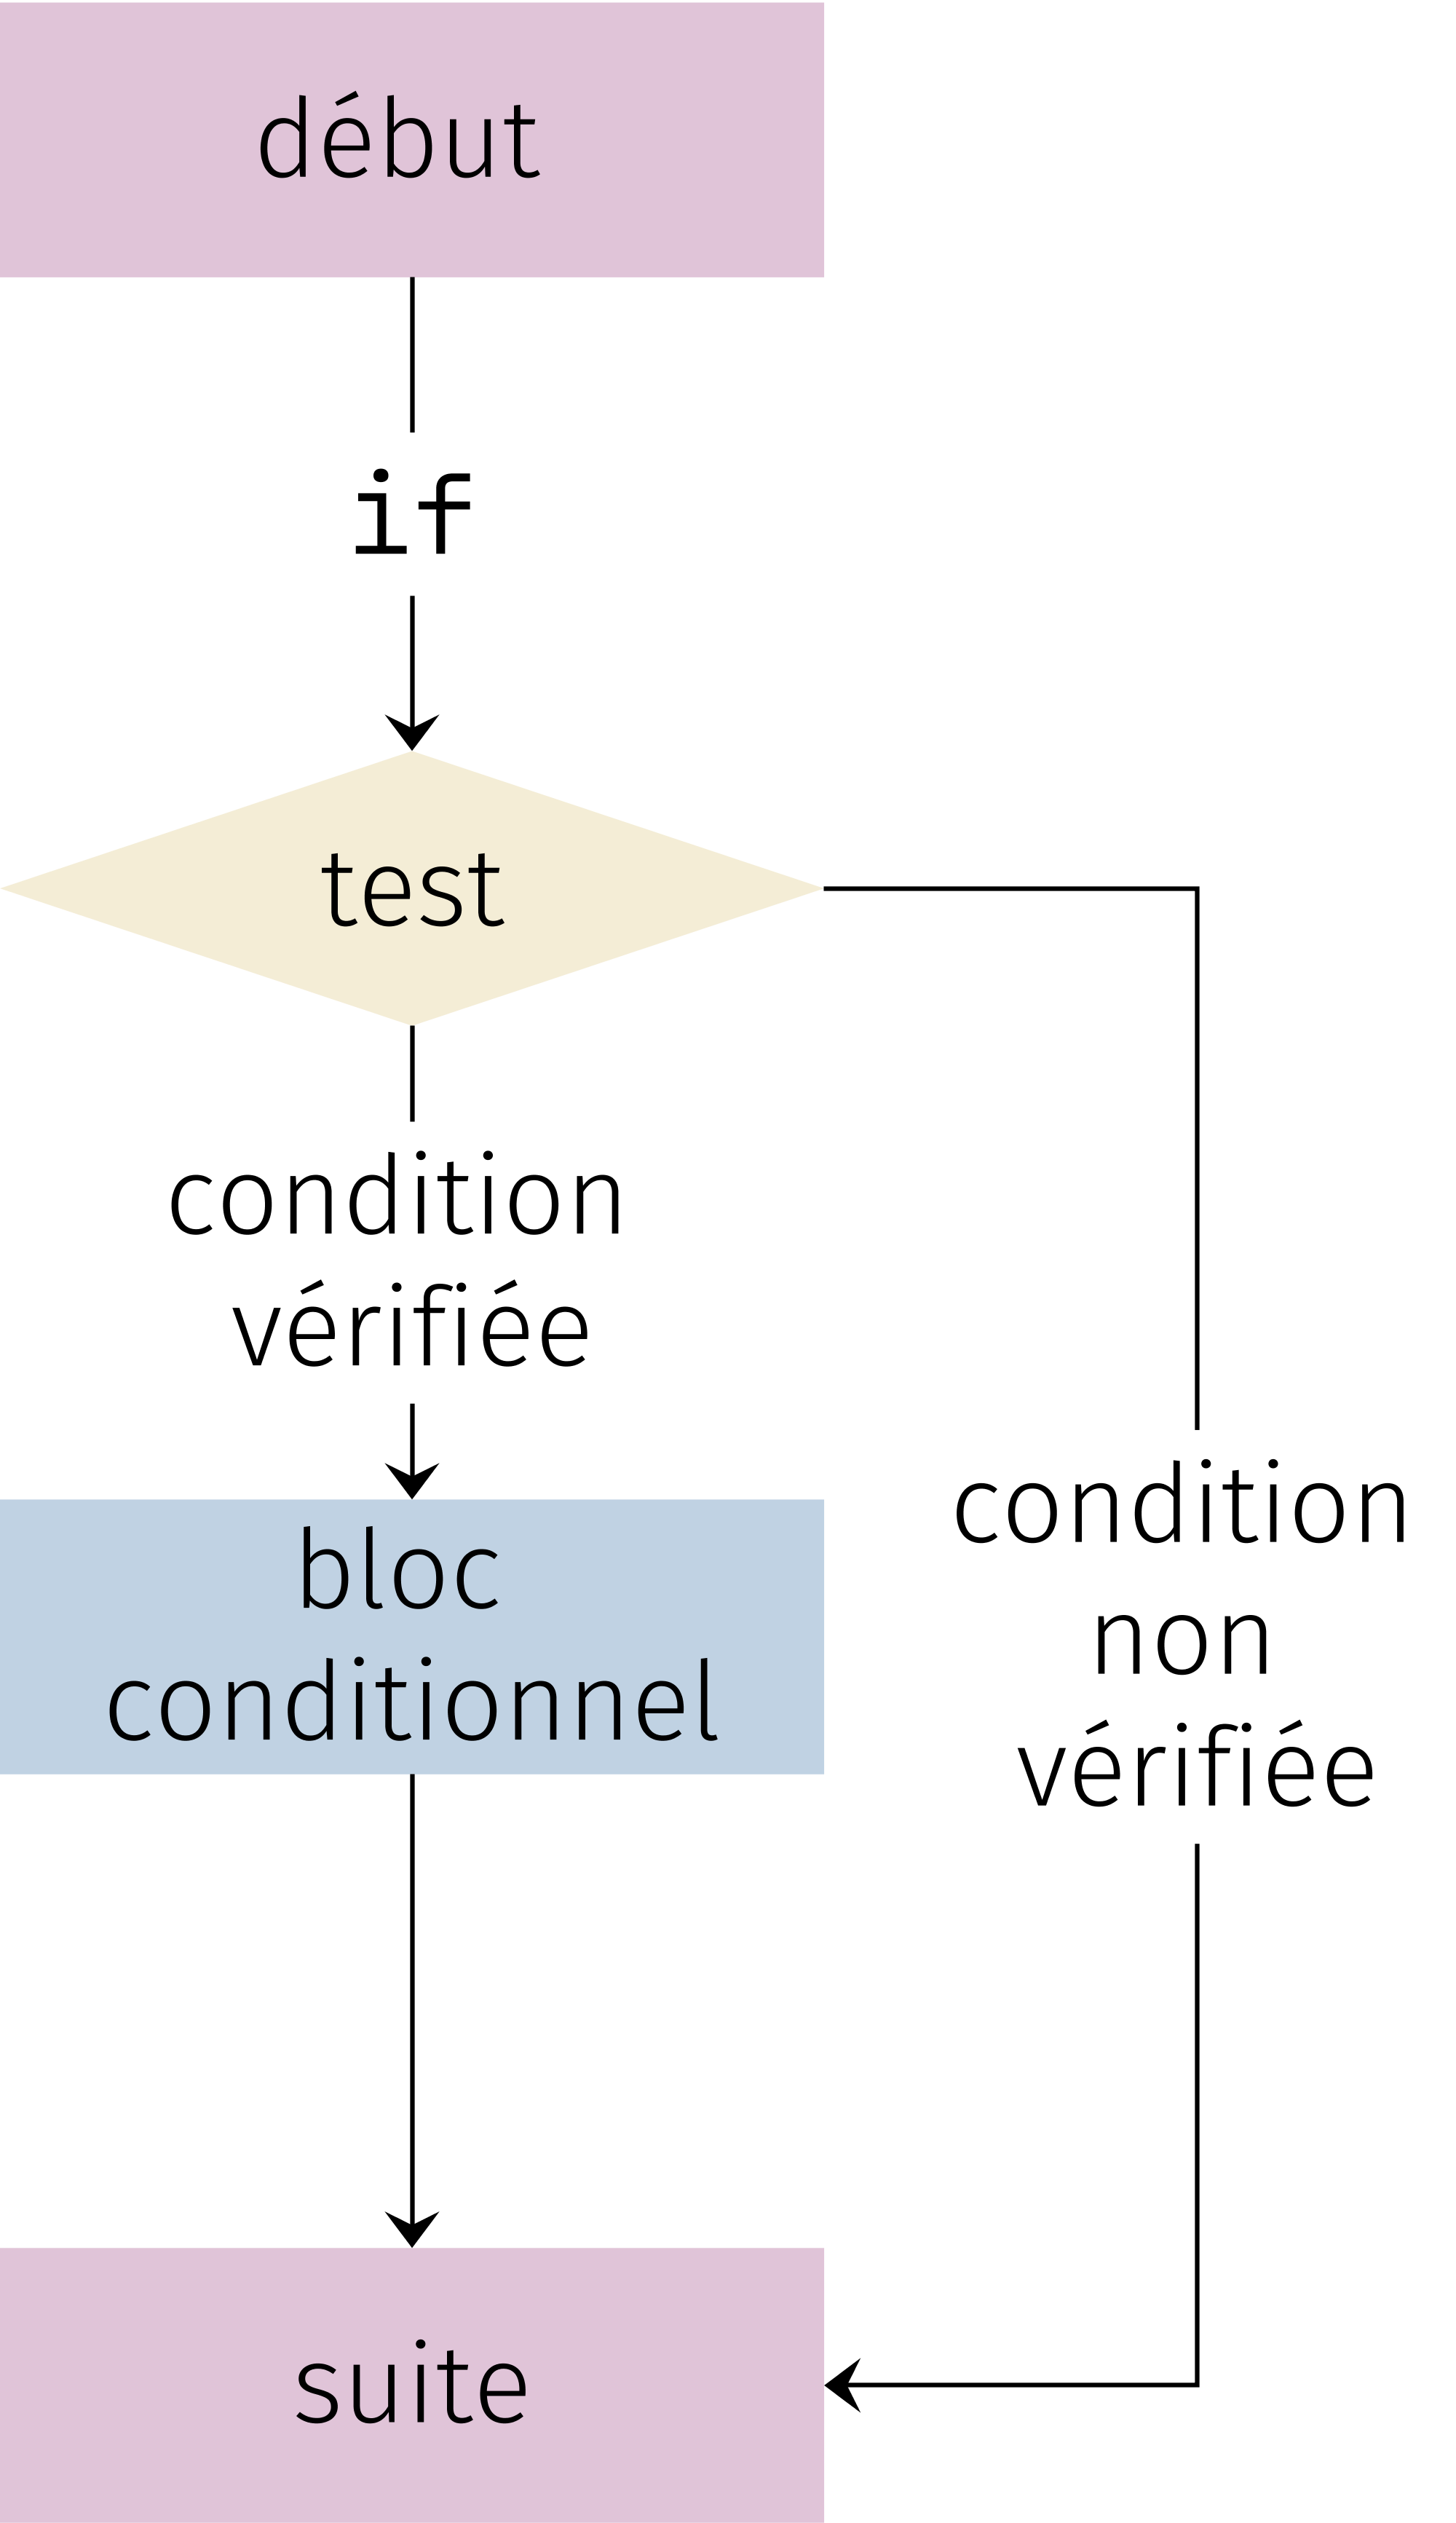
\includegraphics[height=8cm]{ch-conditions/img/if}
\end{center}

\textbf{Attention :} Un bloc conditionnel doit être \textit{tabulé} par rapport à la ligne précédente : il n'y a ni \mintinline{python}{DébutSi}  ni \mintinline{python}{FinSi}
en \textsc{Python}, ce sont les tabulations qui délimitent les blocs.

\begin{pyc}
	\begin{minted}{python}
phrase ='Je vous trouve très joli'
reponse = input('Etes vous une femme ?(O/N) : ')
if reponse == 'O': 
    phrase += 'e' # remarquer la tabulation de cette ligne
phrase +='.'
print(phrase)
\end{minted}
\end{pyc}

Voici le schéma de fonctionnement d'un test \mintinline{python}{if...else} :
\begin{center}
	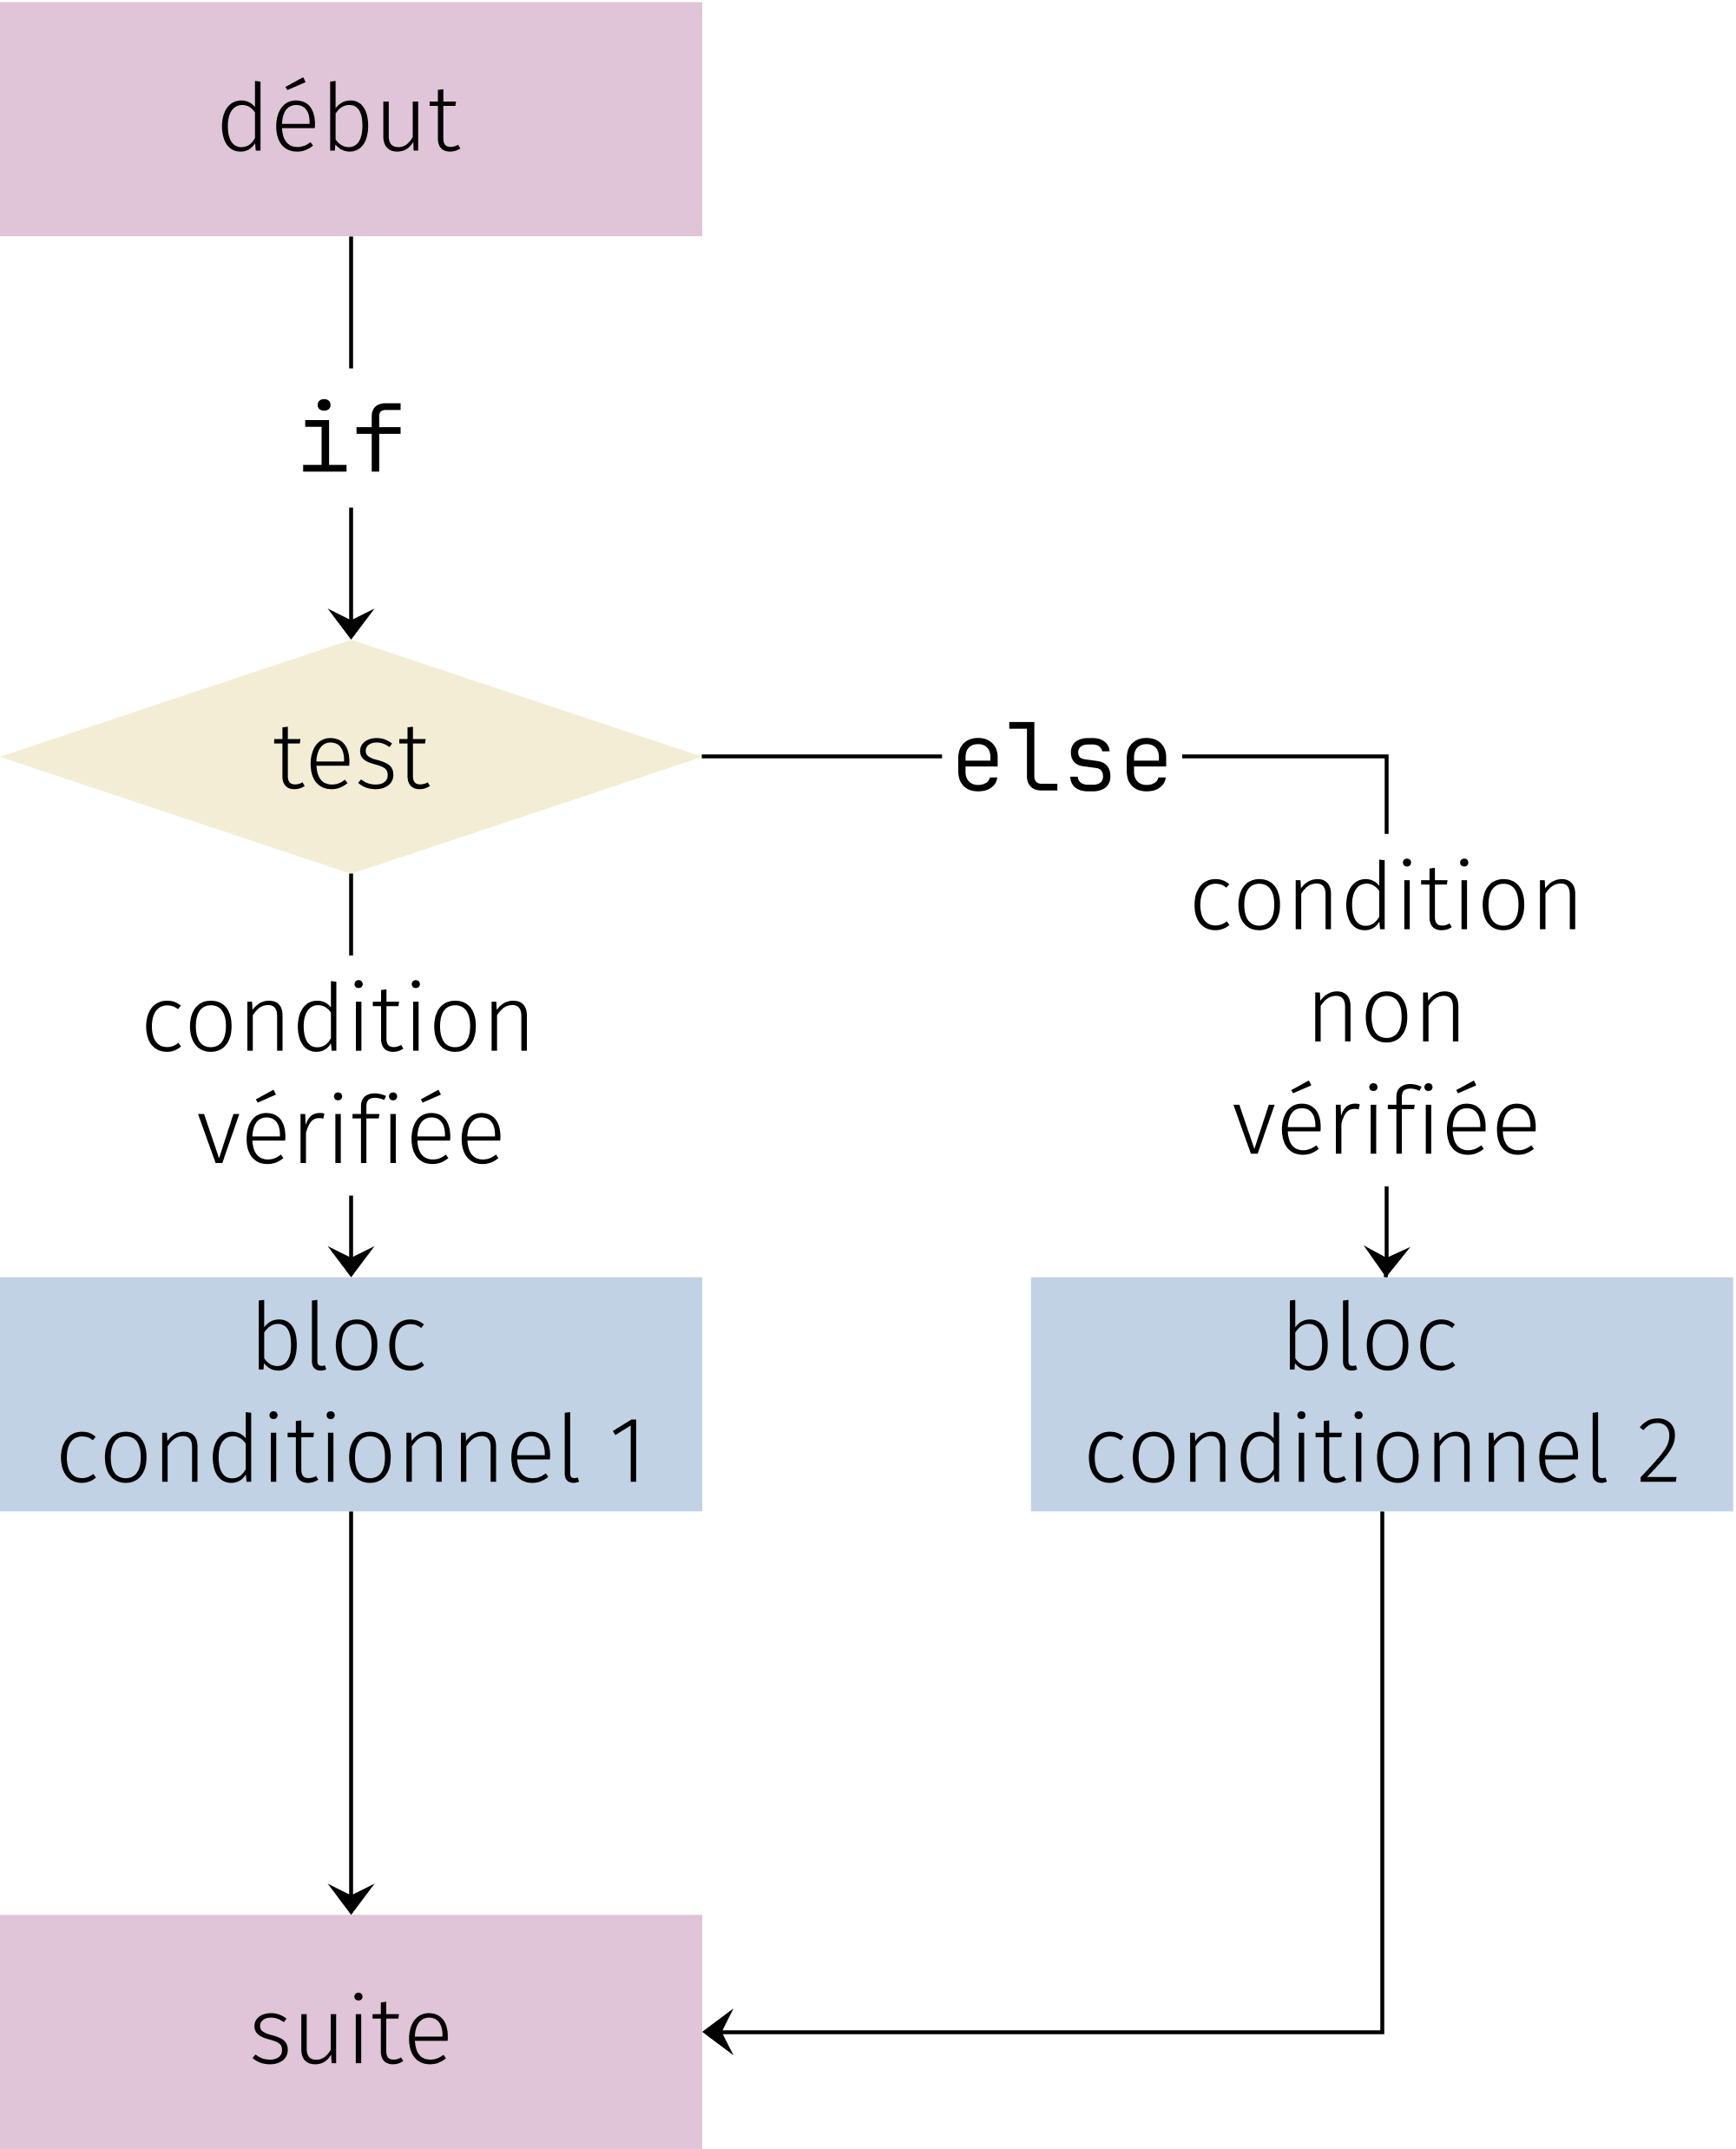
\includegraphics[height=8cm]{ch-conditions/img/ifelse}
\end{center}

\begin{pyc}
	\begin{minted}{python}
print('Bonjour')
age = int(input('Entrez votre age : '))
if age >= 18:
    print('Vous etes majeur')
else:
    print('Vous etes mineur.')
print('Au revoir.')
\end{minted}
\end{pyc}

Voici un exemple de fonctionnement d'un test \mintinline{python}{if...elif...} :
\begin{pyc}
	\begin{minted}{python}
print('Bonjour')
prenom = input('Entrez un prénom : ')
if prenom == 'Robert':
    print("Robert, c'est le prénom de mon grand-père.")
elif prenom == 'Raoul':
    print("Mon oncle s'appelle Raoul.")
elif prenom == 'Médor':
    print("Médor, comme mon chien !")
else:
    print("Connais pas")
print('Au revoir.')
\end{minted}
\end{pyc}
Et voici un schéma décrivant son fonctionnement :
\begin{center}
	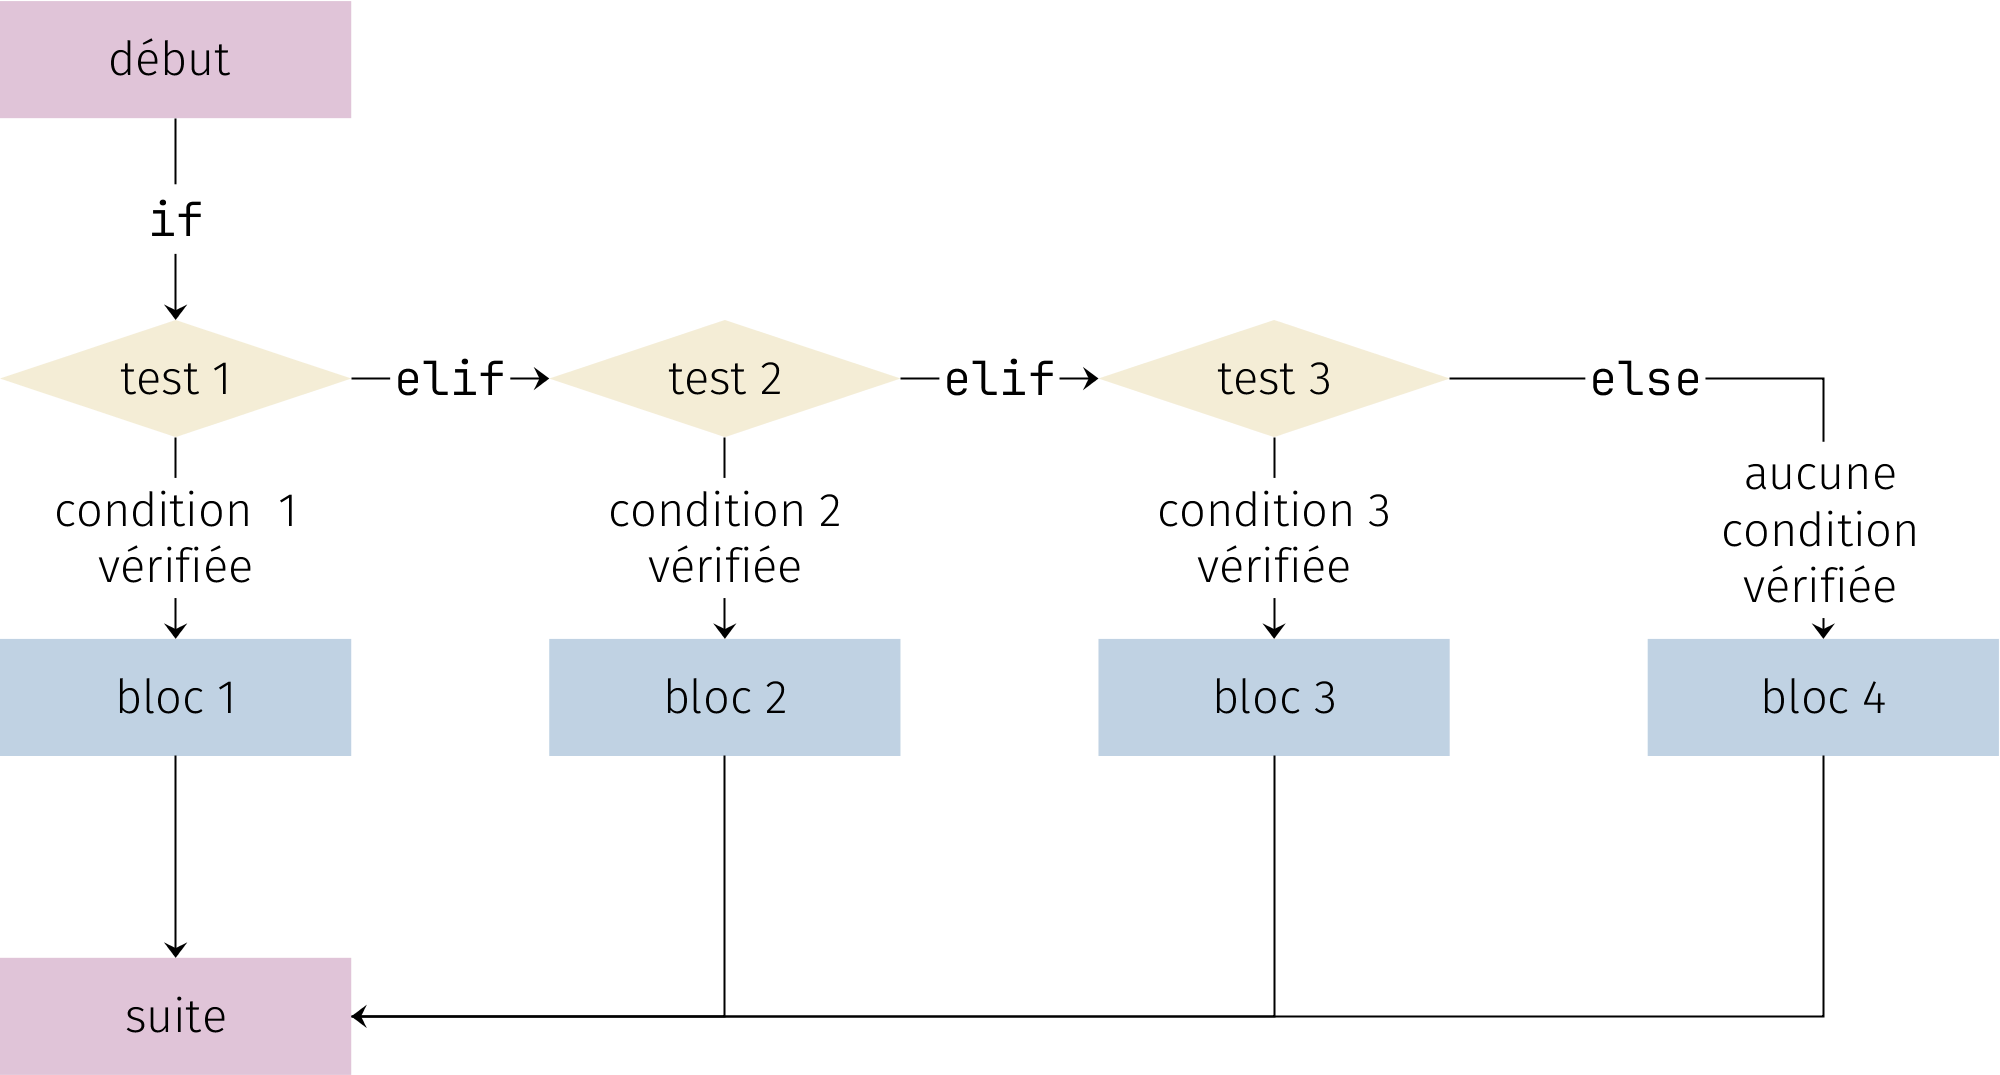
\includegraphics[width=\linewidth]{ch-conditions/img/ifelifelse}
\end{center}



On peut bien sûr inclure autant de \mintinline{python}{elif} que nécessaire.

\section{Exercices}

%----------------------------------------------------------------------
\begin{exercice}
	\'Ecrire un script qui demande son âge à l'utilisateur puis qui affiche \mintinline{python}{'Bravo pour votre longévité.'} si celui-ci est supérieur à 90.
\end{exercice}

\begin{exercice}[]
	\'Ecrire un script qui demande un nombre à l'utilisateur puis affiche si ce nombre est pair ou impair.
\end{exercice}
%----------------------------------------------------------------------
\begin{exercice}
	\'Ecrire un script qui demande l'âge d'un enfant à l'utilisateur puis qui l'informe ensuite de sa catégorie :
	\begin{itemize}
		\item   trop petit avant 6 ans;
		\item   poussin de 6 à 7 ans inclus;
		\item   pupille de 8 à 9 ans inclus;
		\item   minime de 10 à 11 ans inclus;
		\item   cadet à 12 ans et plus;
	\end{itemize}
\end{exercice}
%----------------------------------------------------------------------

\begin{exercice}
	\'Ecrire un script qui demande une note sur 20 à l'utilisateur puis vérifie qu'elle est bien comprise entre 0 et 20. Si c'est le cas rien ne se produit mais sinon le programme devra afficher un message tel que \mintinline{python}{'Note non valide.'}.
\end{exercice}

\begin{exercice}
	\'Ecrire un script qui demande un nombre à l'utilisateur puis affiche s'il est divisible par 5, par 7 par aucun ou par les deux de ces deux nombres.
\end{exercice}
%----------------------------------------------------------------------
\begin{exercice}
	En reprenant l'exercice du chapitre 1 sur les numéros de sécurité sociale, écrire un script qui demande à un utilisateur son numéro de sécurité sociale, puis qui vérifie si la clé est valide ou non.
\end{exercice}


%----------------------------------------------------------------------
\begin{exercice}
	\'Ecrire un script qui résout dans $\R$ l'équation du second degré $ax^2+bx+c=0$.\\
	On commencera par \mintinline{python}{from math import sqrt} pour utiliser la fonction \mintinline{python}{sqrt}, qui calcule la racine carrée d'un \mintinline{python}{float}.
	
	On rappelle que lorsqu'on considère une équation du type $ax^2+bx+c=0$
	\begin{itemize}
		\item   si $a=0$ ce n'est pas une équation de seconde degré;
		\item   sinon on calcule $\Delta = b^2-4ac$ et
		      \begin{itemize}
			      \item   Si $\Delta<0$ l'équation n'a pas de solutions dans $\R$;
			      \item   Si $\Delta=0$ l'équation admet pour unique solution $\dfrac{-b}{2a}$;
			      \item   Si $\Delta>0$ l'équation admet 2 solutions : $\dfrac{-b-\sqrt{\Delta}}{2a}$ et $\dfrac{-b+\sqrt{\Delta}}{2a}$.
		      \end{itemize}
	\end{itemize}
	Pour vérifier que le script fonctionne bien on pourra tester les équations suivantes :
	\begin{itemize}
		\item   $2x^2+x+7=0$ (pas de solution dans $\R$);
		\item   $9x^2-6x+1=0$ (une seule solution qui est $\dfrac{1}{3}$);
		\item   $x^2-3x+2$ (deux solutions qui sont 1 et 2).
	\end{itemize}
\end{exercice}

%----------------------------------------------------------------------
\begin{exercice}
	L'opérateur \mintinline{python}{nand} est défini de la manière suivante : si \mintinline{python}{A} et \mintinline{python}{B} sont deux booléens alors
	\begin{center}
		\mintinline{python}{A nand B} vaut \mintinline{python}{not (A and B)}
	\end{center}
	Construire la table de vérité de \mintinline{python}{nand} en complétant :
	\begin{center}
		\tabstyled
		\begin{tabular}{|c|c|c|c|}
			\hline
			\ccell A                   & \ccell B                   & \ccell A and B & \ccell not (A and B) \\
			\hline
			\mintinline{python}{False} & \mintinline{python}{False} &                &                      \\
			\hline
			\mintinline{python}{False} & \mintinline{python}{True}  &                &                      \\
			\hline
			\mintinline{python}{True}  & \mintinline{python}{False} &                &                      \\
			\hline
			\mintinline{python}{True}  & \mintinline{python}{True}  &                &                      \\
			\hline
		\end{tabular}
	\end{center}
\end{exercice}



% \chapter{Boucles}
\introduction{Tant que tu n'y arrives pas recommence.}
On s'intéresse dans ce chapitre aux \textit{structures itératives}, plus communément appelée \textit{boucles}.\\


\section{La boucle while}

Voici son schéma de fonctionnement :
\begin{center}
    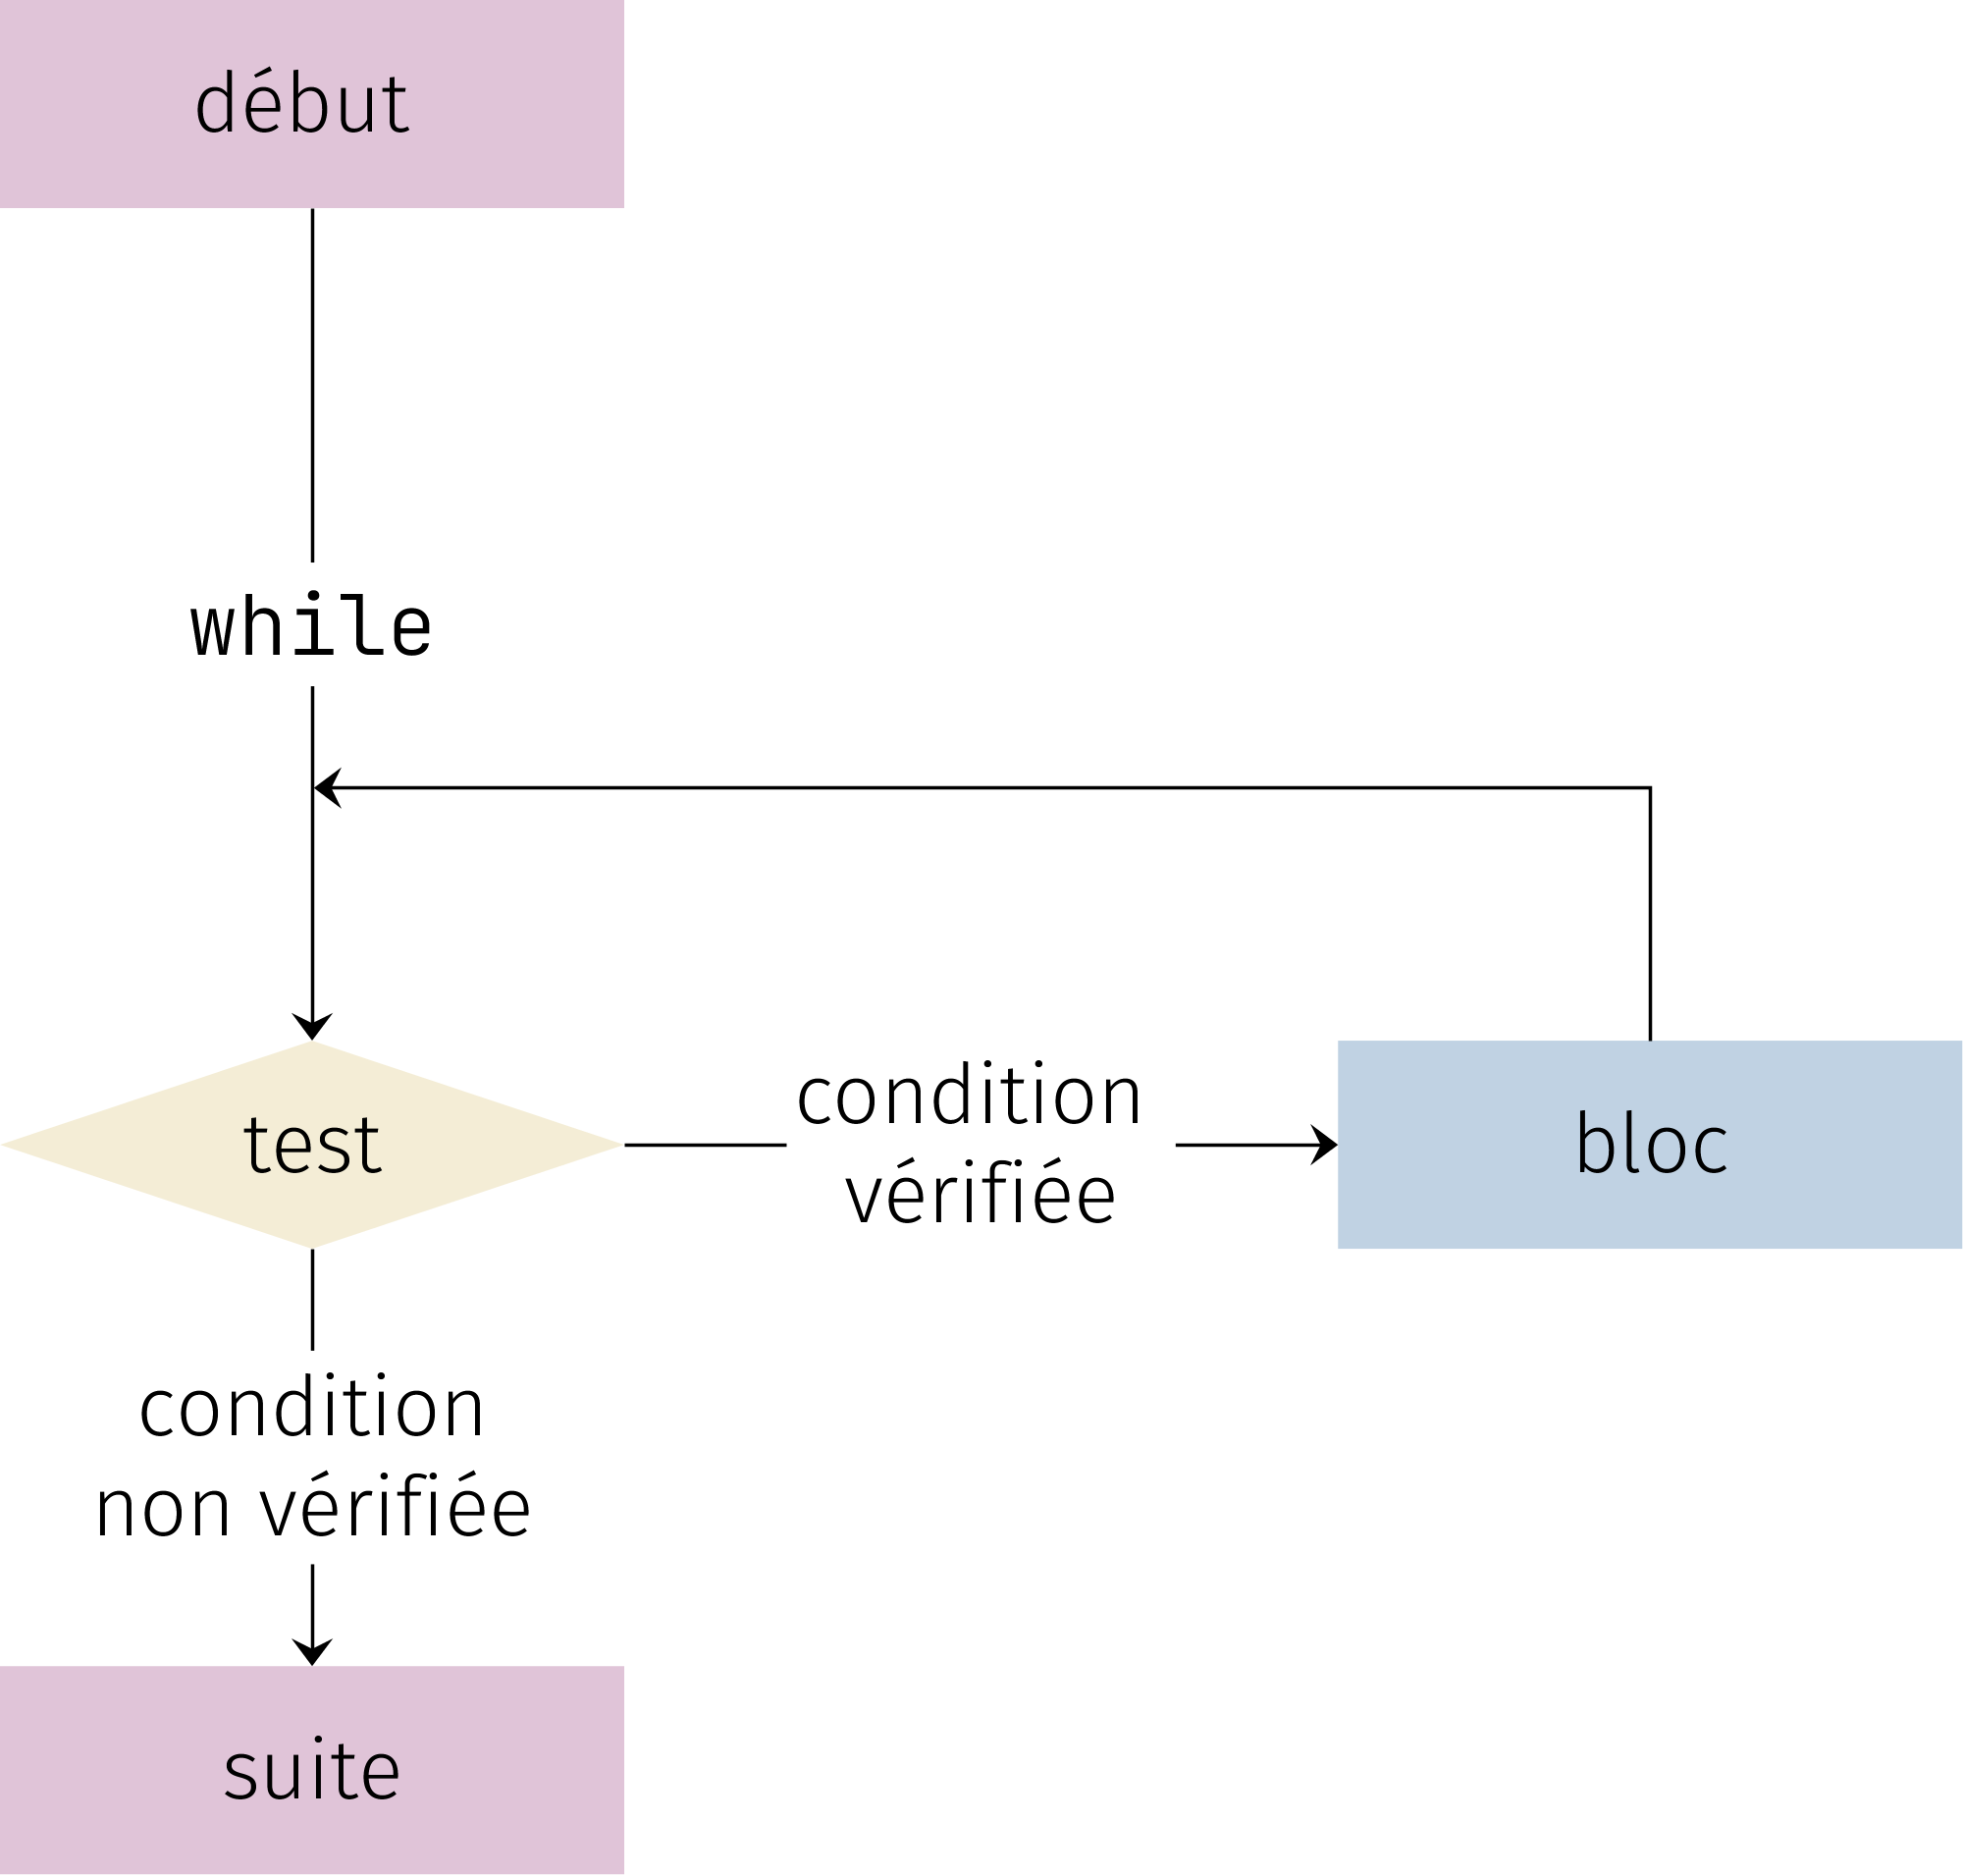
\includegraphics[height=7.5cm]{ch-boucles/img/while.png}
\end{center}

La boucle \mintinline{python}{while} exécute un bloc d'instructions conditionnel \textit{tant que} une condition est vérifiée.\\
Dès que la condition n'est plus vérifiée, le bloc conditionnel n'est plus exécuté.

\begin{pyc}
\begin{minted}{python}
reponse=''
print('Bonjour !')
while reponse !='n':
    reponse = input('Voulez-vous continuer ? (o/n) : ')
print('Au revoir.')
\end{minted}
\end{pyc}
La boucle \mintinline{python}{while} doit être utilisée avec soin : si la condition est toujours vérifiée, le programme ne s'arrêtera pas :

\begin{pyc}
\begin{minted}{python}
while True:
    print('Au secours !')
\end{minted}
\end{pyc}
Voici un exemple typique d'utilisation de la boucle \mintinline{python}{while} : \\

On place un capital de 2000 euros sur un compte à intérêts annuels de 2\%. On aimerait savoir au bout de combien de temps, sans rien toucher, le 
solde du compte dépassera 2300 euros.\\

\begin{pyc}
\begin{minted}{python}
solde = 2000  # solde initial
n = 0  # nombre d'annees
while solde <= 2300:  # condition de boucle
    n += 1  # augmente le compteur d'annees
    solde *= 1.02  # actualise le solde
print(' Il nous faudra ', n, 'ans.')  # affichage final   
\end{minted}
\end{pyc}

\section{La boucle for ... in range(...)}

Commençons par examiner un nouveau type : \mintinline{python}{range} (plage de valeurs)

\begin{pyc}
\begin{minted}{python}
>>> a = range(10)
>>> type(a)
>>> print(list(a))
\end{minted}
\end{pyc}

Si \mintinline{python}{range(10)} ressemble beaucoup à la liste \mintinline{python}{[0,1,...,9]}, la finalité de \\\mintinline{python}{range(10)} est d'être un \textit{itérateur}, 
c'est-à-dire une objet dont on peut parcourir le contenu pour créer une boucle :

\begin{pyc}
\begin{minted}{python}
for i in range(10):
    print(i)
\end{minted}
\end{pyc}
La syntaxe complète de \mintinline{python}{range} est : \mintinline{python}{range(<debut>,fin,<increment>)}.\\

Par défaut, si ce n'est pas précisé, \mintinline{python}{debut=0}, et \mintinline{python}{increment=1}.\\

\mintinline{python}{range(<debut>,fin,<increment>)} renvoie la plage de valeurs suivantes :
\begin{itemize}
    \item   On part de la valeur de début, appelons la \mintinline{python}{val}
    \item   Tant que \mintinline{python}{val < fin}:\\
    $\qquad$ - ajouter \mintinline{python}{val} à la plage\\
    $\qquad$ - ajouter \mintinline{python}{increment} à \mintinline{python}{val}
\end{itemize}
Ainsi, \mintinline{python}{range(2,52,10)} renvoie la plage de valeurs \mintinline{python}{2,12,22,32,42}, mais\\ \mintinline{python}{range(2,53,10)} renvoie la plage de valeurs 
\mintinline{python}{2,12,22,32,42,52}.\\

Très souvent, on se contente d'utiliser une instruction du type \mintinline{python}{range(n)}, où \mintinline{python}{n} est de type \mintinline{python}{int}.\\


Voici un exemple : Calculons $1+2+\ldots+100$ :

\begin{pyc}
\begin{minted}{python}
somme = 0
for i in range(1, 101):
    somme += i
print(somme)
\end{minted}
\end{pyc}

\section{La boucle for ... in ...}

On peut généraliser le paragraphe précédent à toute \textit{variable itérable}, c'est extrêmement puissant : les \mintinline{python}{str}, les \mintinline{python}{list} et les 
\mintinline{python}{dict} sont des types itérables.\\

Voici des exemples :\\

Comptons le nombre de voyelles d'une chaîne de caractères :

\begin{pyc}
\begin{minted}{python}
voyelles = 'aeiouy'  # ensemble de voyelles
phrase = input('Entrez une phrases sans accents : ').lower()  # phrase mise en minuscules
compteur = 0  # comptera les voyelles
for lettre in phrase:  # on parcourt la phrase
    if lettre in voyelles:  # est-ce une voyelle ?
        compteur += 1  # si oui on comptabilise
print('Nombre de voyelles : ', compteur)  # affiche le nombre
\end{minted}
\end{pyc}

Faisons la moyenne d'une liste de notes :


\begin{pyc}
\begin{minted}{python}
liste_notes = [12, 11.5, 13, 18, 13, 11, 9]
moyenne = 0
for note in liste_notes:
    moyenne += note
moyenne /= len(liste_notes)
print(moyenne)
\end{minted}
\end{pyc}

Pour le dernier exemple on utilise le type \mintinline{python}{dict} : soit \mintinline{python}{a} une variable de ce type :
\begin{itemize}
    \item   \mintinline{python}{a.keys()} renvoie la liste des clés (des indices du dictionnaire).
    \item   \mintinline{python}{a.values()} renvoie la liste des valeurs prises par le dictionnaire.
\end{itemize}

Voici un second programme de moyenne :

\begin{pyc}
\begin{minted}{python}
resultats = {'EPS': 12, 'maths': 15, 'info': 18}
moyenne = 0
for note in resultats.values():
    moyenne += note
moyenne /= len(resultats)
print(moyenne)
\end{minted}
\end{pyc}

\section{Quelle boucle utiliser ?}

Si la boucle dépend d'une condition particulière on préfèrera la boucle \mintinline{python}{while}.

Si le nombre d'itérations de la boucle est connu on préfèrera une boucle \mintinline{python}{for}.

On peut utiliser une boucle \mintinline{python}{for} sur toute \textit{structure itérative}, par exemple 
    une variable de type \mintinline{python}{range}, \mintinline{python}{str}, \mintinline{python}{list} ou, dans une certaine mesure, \mintinline{python}{dict}.
    
\section{Exercices}
\begin{exercice}
    Calculer à l'aide d'un script la somme des carrés des 1000 premiers entiers non nuls.
\end{exercice}

%----------------------------------------------------------------------
\begin{exercice}
    Calculer à l'aide d'un script la somme des carrés des 1000 premiers multiples de 3 non nuls.
\end{exercice}

%---------------------------------------------------------------------
\begin{exercice}
    \'Ecrire un script qui demande une phrase à l'utilisateur, puis affiche la phrase en rajoutant des tirets.\\
    Exemple : on entre \mintinline{python}{'Salut à toi'} le script affiche \mintinline{python}{'S-a-l-u-t- -à- -t-o-i-}.
\end{exercice}

\begin{exercice}
    Calculer à l'aide d'un script le nombre $n$ à partir duquel la somme $1^2+2^2+\ldots+n^2$ dépasse un milliard.
\end{exercice}

%----------------------------------------------------------------------
\begin{exercice}
    \'Ecrire un script qui demande une phrase et compte le nombre d'occurrences de la lettre  «  a  »  dans celle-ci.
\end{exercice}

%----------------------------------------------------------------------
\begin{exercice}
    Programmer le jeu du "plus petit plus grand" :
    \begin{itemize}
        \item   L'ordinateur choisit un nombre entier au hasard compris entre 0 et 100.\\
        Au début du script, importer la fonction \mintinline{python}{randint} du module \mintinline{python}{random} avec \mintinline{python}{form random import randint}.\\
        Pour obtenir un entier au hasard, utiliser \mintinline{python}{randint(0,100)}.
        \item   L'utilisateur propose un nombre, l'ordinateur répond  «  gagné » ,  «  plus petit »  ou  «  plus grand » .
        \item   Le programme continue tant que l'utilisateur n'a pas gagné.
    \end{itemize}
\end{exercice}

%----------------------------------------------------------------------
\begin{exercice}
    On considère la suite $s$ définie par:
    \tabulardefault
    $$\left\lbrace 
    \begin{array}{llll}
    s_0 & = & 1000 & \\
    s_{n+1} & = & 0,99s_n+1 & \textrm{pour tout } n\in\mathbf{N}
    \end{array}
    \right. $$
    
    \begin{itemize}
        \item   \'Ecrire un script calculant les premiers termes de $s$ (vous décidez le nombre de termes).
        \item   Utiliser ce script pour conjecturer la limite de $s$.
        \item   Modifier ce script pour obtenir le plus petit entier $n$ tel que l'écart entre $s_n$ et sa limite soit inférieur ou égal à $10^{-4}$.
        
    \end{itemize}
\end{exercice}

%----------------------------------------------------------------------
\begin{exercice}
    $\varphi$ (lettre phi, équivalent du  «  f  »  en grec) est défini par : $$\varphi=1+\frac{1}{1+\frac{1}{1+\frac{1}{\ldots}}}$$
    Sur papier, fabriquer une suite par récurrence commençant ainsi :
    \begin{itemize}
        \item   1
        \item   $1+\frac{1}{1}$
        \item   $1+\frac{1}{1+\frac{1}{1}}$
        \item   Et c\ae tera (trouver une relation simple pour calculer le terme suivant à partir du terme actuel).
    \end{itemize}
    Programmer un script qui calcule successivement les termes de cette suite (aller jusqu'à 10000\eme).\\
    
    Comparer avec la valeur exacte de $\varphi$, qui est $\frac{1+\sqrt{5}}{2}$.
\end{exercice}

\begin{exercice}
    \'Ecrire un script qui détermine si un entier est premier ou pas.
\end{exercice}
% \chapter{Listes}
\label{ch:listes}
Le type \mintinline{python}{list} permet de stocker des valeurs dans un ordre précis.
\begin{pyc}
	\begin{minted}{python}
		# on crée une liste avec 3 valeurs
		lst = ['bonjour', 3.14, True]
	\end{minted}
\end{pyc}
Une valeur de type \mintinline{python}{list} est itérable :
\begin{itemize}
	\item on peut accéder à un élément de la liste, par exemple \mintinline{python}{lst[0]} ;
	\item on peut parcourir une liste.
\end{itemize}

Pour accéder à un élement d'une liste situé à un endroit précis, on doit connaître son \textit{indice} : le premier élément d'une liste a l'indice zéro, le deuxième l'indice 1, \textit{et cætera}.

\begin{pyc}
	\begin{minted}{python}
		# on crée une liste avec 3 valeurs
		>>> lst = ['bonjour', 3.14, True]
		# premier élément : indice 0
		>>> lst[0]
		'bonjour'

		# deuxième élément
		>>> lst[1] 
		3.14
	\end{minted}
\end{pyc}

\section{Opérations de base}

\subsection{Créer une liste}

\begin{itemize}
	\item \mintinline{python}{lst = list()} crée une liste vide ;
	\item \mintinline{python}{lst = []} fait la même chose ;
	\item  \mintinline{python}{lst = ['a', 7, True]} crée une liste composée de 3 éléments.
\end{itemize}
Une liste peut contenir des éléments de plusieurs types mais en pratique on évite cela.


\subsection{Modifier un élément}
Le type \mintinline{python}{list} est \textit{mutable} : on peut changer un ou des éléments d'une liste \textit{sans changer la liste elle-même}.

\begin{pyc}
	\begin{minted}{python}
		>>> lst = [2, 3, 4, 1]
		# on change le deuxième élément
		>>> lst[1] = 10
		>>> lst
		[2, 10, 4, 1]
	\end{minted}
\end{pyc}
\subsection{Ajouter un élément en fin de liste}

On reprend l'exemple précédent

\begin{pyc}
	\begin{minted}{python}
		>>> lst.append(7) # ajoute 7 à la fin de la liste
		>>> lst
		[2, 10, 4, 1, 7]
	\end{minted}
\end{pyc}

\begin{remarque}
	\mintinline{python}{lst = lst + [7]} a le même effet  que \mintinline{python}{lst.append(7)} : on crée une « mini-liste » \mintinline{python}{[4]}, on concatène les 2 listes et on remet le résultat dans \mintinline{python}{lst}.\\
	En pratique la première méthode est la plus simple et aussi la plus rapide.
\end{remarque}

\subsection{Insérer un élément à une place donnée}

Pour une liste \mintinline{python}{lst} valant \mintinline{python}{[2, 10, 4, 1]}, si on veut insérer la valeur 5 à l'indice 1 on écrira :\\

\mintinline{python}{lst.insert(1, 5)} \\

et \mintinline{python}{lst} vaudra \mintinline{python}{[2, 5, 10, 4, 1]}\\

La syntaxe est \mintinline{python}{lst.insert(indice, valeur)}
\subsection{Retirer un élément à une position donnée}
Si une liste \mintinline{python}{lst} a pour valeur \mintinline{python}{[3 ,7, 1]} et qu'on veut supprimer son deuxième élément alors on écrit :\\

\mintinline{python}{del lst[1]}\\

Ensuite, \mintinline{python}{lst} aura la valeur \mintinline{python}{[3,1]}.

\subsection{Retirer une valeur précise}
Pour retirer une valeur \textit{qui appartient à une liste} on procède ainsi :\\

Si \mintinline{python}{lst} a la valeur \mintinline{python}{[1, 2, 5, 4, 2, 3]} alors l'instruction \\

\mintinline{python}{lst.remove(2)}\\

Supprime la \textit{première occurrence} de \mintinline{python}{2} dans \mintinline{python}{lst}.\\
Après cela, \mintinline{python}{lst} a la valeur \mintinline{python}{[1, 5, 4, 2, 3]}.


\subsection{Concaténer des listes}
On peut procéder de 2 manières :
\begin{itemize}
	\item \mintinline{python}{lst1.extend(lst2)} ajoute les éléments de la liste \mintinline{python}{lst2} à la fin de \mintinline{python}{lst1} ;
	\item \mintinline{python}{lst1 = lst1 + lst2} crée une liste avec les éléments de \mintinline{python}{lst1} et ceux de \mintinline{python}{lst2}, puis replace le résultat dans \mintinline{python}{lst1}.
\end{itemize}
En pratique la première méthode est plus rapide.


\subsection{Longueur d'une liste}
La fonction \mintinline{python}{len}
\begin{itemize}
	\item prend en entrée une liste \mintinline{python}{lst} ;
	\item renvoie la longueur de cette liste.
\end{itemize}

Ainsi \mintinline{python}{len([2, 3, 4])} vaut 3.

\subsection{Divers}
\mintinline{python}{lst.sort()} trie la liste dans l'ordre croissant.\\

\mintinline{python}{lst.reverse()} met les éléments dans l'ordre inverse.

\section{Opérations avancées}


\subsection{Copier une liste (mauvaise méthode)}
\begin{pyc}
	\begin{minted}{python}
>>> lst1 = [5, 6, 8]
>>> lst2 = lst1
>>> lst1[0] = 10
>>> lst1
[10, 6, 8]

>>> lst2
[10, 6, 8]  # problème : lst2[0] a changé aussi !
\end{minted}
\end{pyc}

Ce comportement « étrange » vient du fait que le type \mintinline{python}{list} est \textit{mutable}. Nous allons expliquer cela plus tard dans ce chapitre.

\subsection{Copier une liste (bonne méthode)}
\begin{pyc}
	\begin{minted}{python}
>>> lst1 = [5, 6, 8]
>>> lst2 = lst1[:] # on copie tous les éléments de lst1 dans lst2
>>> lst1[0] = 10
>>> lst1
[10, 6, 8]

>>> lst2
[5, 6, 8] # Ouf !
\end{minted}
\end{pyc}

\subsection{Extraire une sous-chaîne}
Soit \mintinline{python}{lst} une liste de longueur $n$ et $p$ et $q$ deux entiers tels que $0\leqslant p <q\leqslant n$ . Alors
\begin{itemize}
	\item \mintinline{python}{lst[p:q]} est la liste composée des éléments \mintinline{python}{lst[p]}, \ldots, \mintinline{python}{lst[q-1]} ;
	\item \mintinline{python}{lst[:q]} signifie \mintinline{python}{lst[0:q]} ;
	\item \mintinline{python}{lst[p:]} signifie \mintinline{python}{lst[p:n]}.
\end{itemize}




\begin{exemple}[]
	Si \mintinline{python}{lst} vaut \mintinline{python}{[2, 5, 3, 4, 9, 2, 5]} alors
	\begin{itemize}
		\item \mintinline{python}{lst[2:6]} vaut \mintinline{python}{[3, 4, 9, 2]} ;
		\item \mintinline{python}{lst[3:]} vaut \mintinline{python}{[4, 9, 2, 5]} ;
		\item \mintinline{python}{lst[:2]} vaut \mintinline{python}{[2, 5]}.
	\end{itemize}
\end{exemple}




\section{Parcourir une liste}
\subsection{Parcours selon les indices}

\begin{definition}[ : parcours selon les indices]
	Soit \mintinline{python}{lst} une liste de longueur \mintinline{python}{n}.\\

	Alors ses éléments sont \mintinline{python}{lst[0]}, \ldots, \mintinline{python}{lst[n-1]} et on parcourt la liste en
	\begin{itemize}
		\item considérant un entier \mintinline{python}{i} qui jouera le rôle d'\textit{indice} ;
		\item faisant parcourir à \mintinline{python}{i} la plage de valeurs \mintinline{python}{range(n)} ;
		\item considérant les \mintinline{python}{lst[i]}.
	\end{itemize}
\end{definition}
\begin{exemple}[ : un parcours selon les indices]
	On affiche les élements d'une liste grâce à un parcours par les indices.
	\begin{minted}{python}
	lst = [54, 65, 123]
	n = len(lst) # n vaut 3
	for i in range(n): # range(3), c'est 0, 1, 2
		print(lst[i])
	\end{minted}
\end{exemple}

Le parcours d'une liste par les indices est \textit{crucial} lorsque lors du parcours, on veut savoir à quelle place on se trouve dans la liste. C'est le cas quand on veut déterminer si une liste est triée dans l'ordre croissant ou non : il faut regarder si chaque élement est plus petit que le suivant dans la liste.\\
C'est aussi le cas quand on veut par exemple déterminer l'indice de la première apparition d'une valeur dans une liste.


\subsection{Parcours selon les éléments}

C'est plus simple que le parcours selon les indices mais on pert un peu d'information car pendant le parcours, on ne sait pas à quelle place on se trouve dans la liste.

\begin{definition}[ : parcours selon les éléments]
	Le parcours des éléments d'une liste \mintinline{python}{lst} s'effectue à l'aide d'une simple boucle \mintinline{python}{for x in lst}. \mintinline{python}{x} prend alors successivement les valeurs de chacun des éléments de \mintinline{python}{lst}, dans l'ordre.
\end{definition}
\begin{exemple}[ : un parcours selon les éléments]
	\begin{minted}{python}
		lst = [54, 65, 123]
		for x in lst:
			print(x)
		\end{minted}
\end{exemple}

\subsection{Bilan}

On peut toujours utiliser un parcours de liste selon les indices.
On peut toujours transformer un parcours selon les éléments en un parcours selon les indices.
Le contraire est faux si l'on a \textit{absolument} besoin de savoir quels sont les indices des éléments que l'on examine lors du parcours.

\begin{encadrecolore}{À éviter absolument}{UGLiRed}
	Les codes comme celui-ci :
	\begin{minted}{python}
		for i in lst:
			print(i)
	\end{minted}
	On a l'impression que \mintinline{python}{i} est un indice mais c'est une valeur, et l'expérience prouve que dans 90\% des cas, une erreur du type \mintinline{python}{lst[i]} survient, alors que\ldots \mintinline{python}{i} n'est pas un indice ici !\\

	De même les codes comme celui-là :
	\begin{minted}{python}
		for x in range(len(lst)):
			print(lst[x])
	\end{minted}
	Là encore il y a beaucoup de chances que l'indice \mintinline{python}{x} soit pris pour une valeur.
\end{encadrecolore}

\begin{encadrecolore}{Conseil}{UGLiGreen}
	Réserver les noms de variables \mintinline{python}{i}, \mintinline{python}{j} et \mintinline{python}{k} pour les indices et \mintinline{python}{x}, \mintinline{python}{y} et \mintinline{python}{z} pour les éléments.
\end{encadrecolore}

\section{Mutabilité}

Examinons la différence entre un type \textit{non mutable} tel que \mintinline{python}{int} et le type \mintinline{python}{list}, qui est \textit{mutable}.
\subsection{Variables de type non-mutable}

\floatpictureright{0.4}{ch-listes/img/nonmut1}{
	\mintinline{python}{a = 2}\\

	La valeur 2 est stockée en mémoire et une variable \mintinline{python}{a} est créée, associée à cette valeur.
}

\floatpictureleft{0.4}{ch-listes/img/nonmut2}{
	\mintinline{python}{b = a}\\

	Une deuxième variable \mintinline{python}{b} est créée, avec pour valeur 2 également. Elles partagent la même adresse-mémoire.
}

\floatpictureright{0.4}{ch-listes/img/nonmut3}{
	\mintinline{python}{b = 10}\\

	La valeur 10 est stockée dans une autre adresse mémoire (car la valeur 2 sert toujours pour \mintinline{python}{a}) et associée à \mintinline{python}{b}.
}

\subsection{Variables de type mutable}
\subsubsection{Copier une liste (mauvaise méthode)}
\mintinline{python}{lst1 = [5, 6, 8]}\\

Les élements 5, 6 et 8 sont stockés en mémoire et \mintinline{python}{lst1} contient l'adresse du début de la plage mémoire à laquelle ces valeurs sont stockées. \\
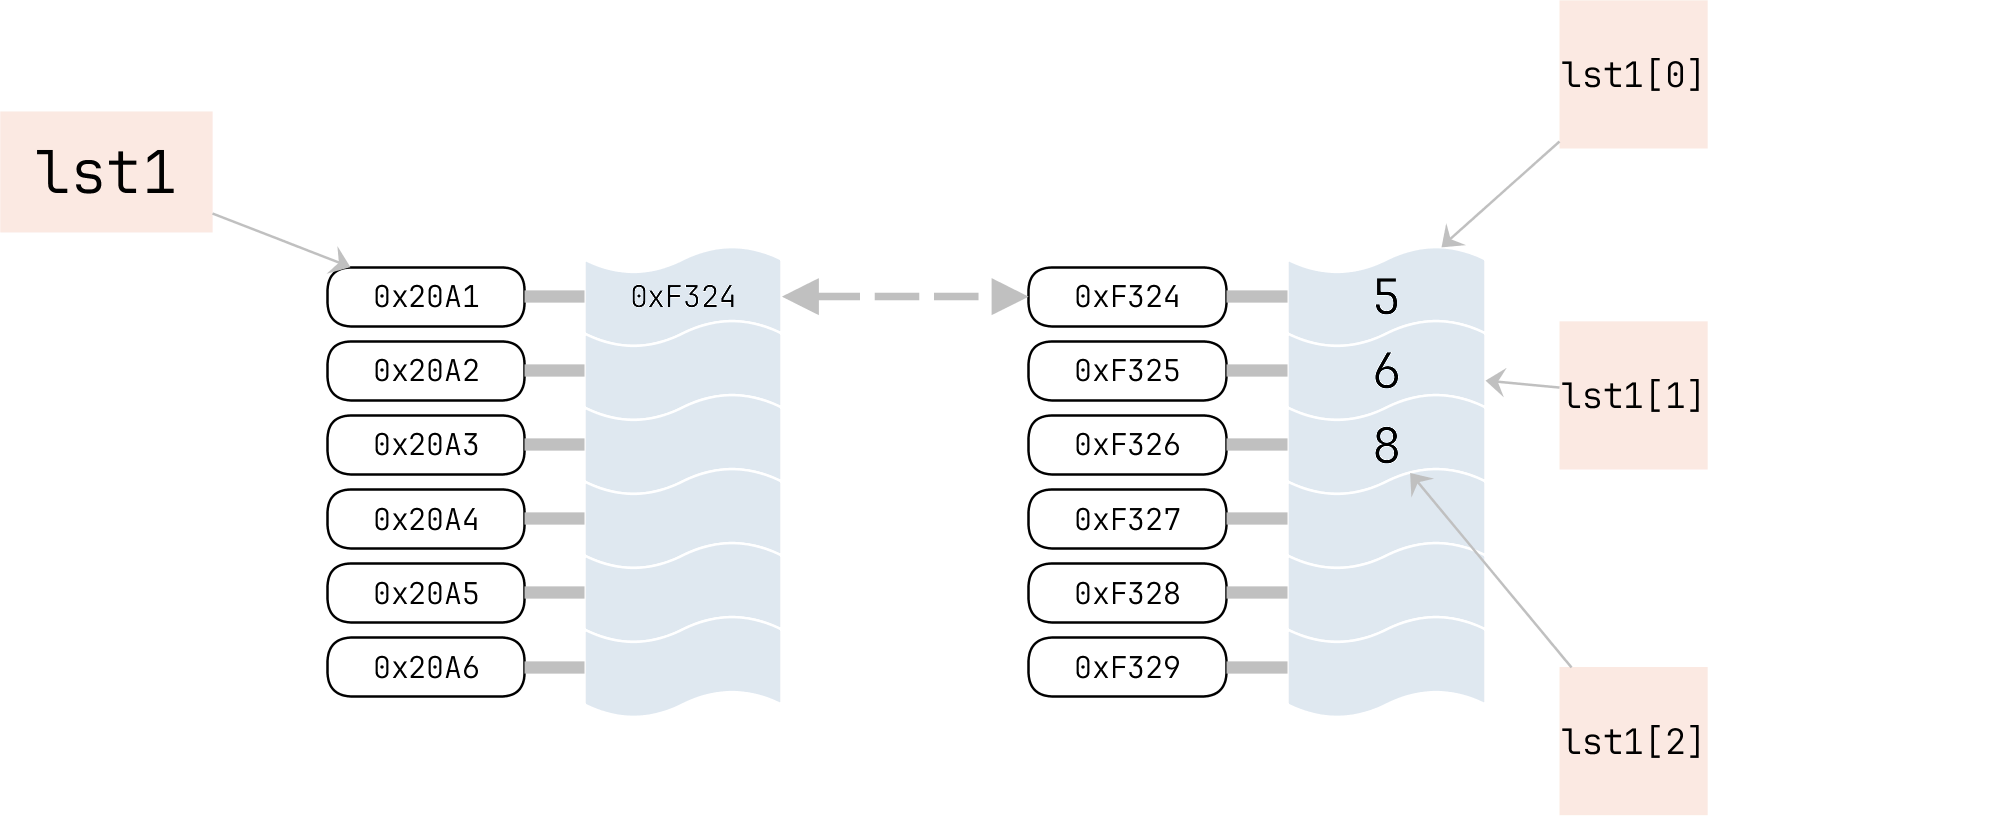
\includegraphics[width=\linewidth]{ch-listes/img/mut1.png}\\


\mintinline{python}{lst2 = lst1}\\

La variable \mintinline{python}{lst2} est associée à la même valeur que \mintinline{python}{lst1}.\\
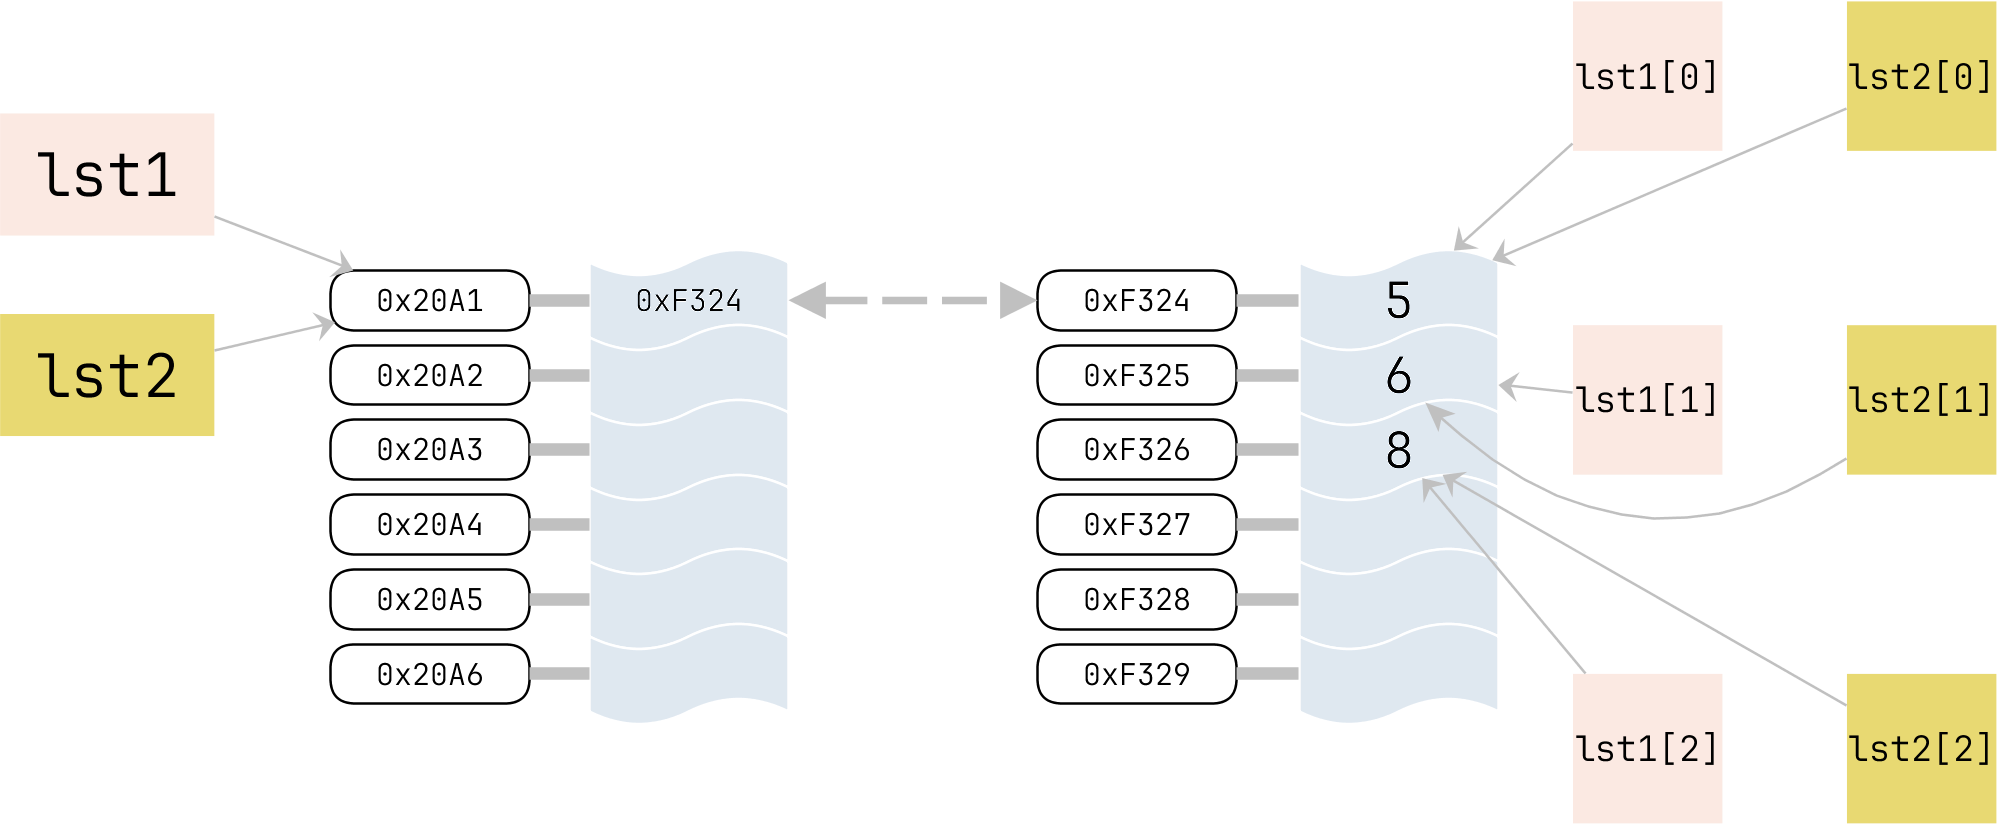
\includegraphics[width=\linewidth]{ch-listes/img/mut2.png}\\


\mintinline{python}{lst1[0] = 10}\\

La valeur de \mintinline{python}{lst1[0]} est changée, elle l'est donc aussi pour \mintinline{python}{lst2}.\\
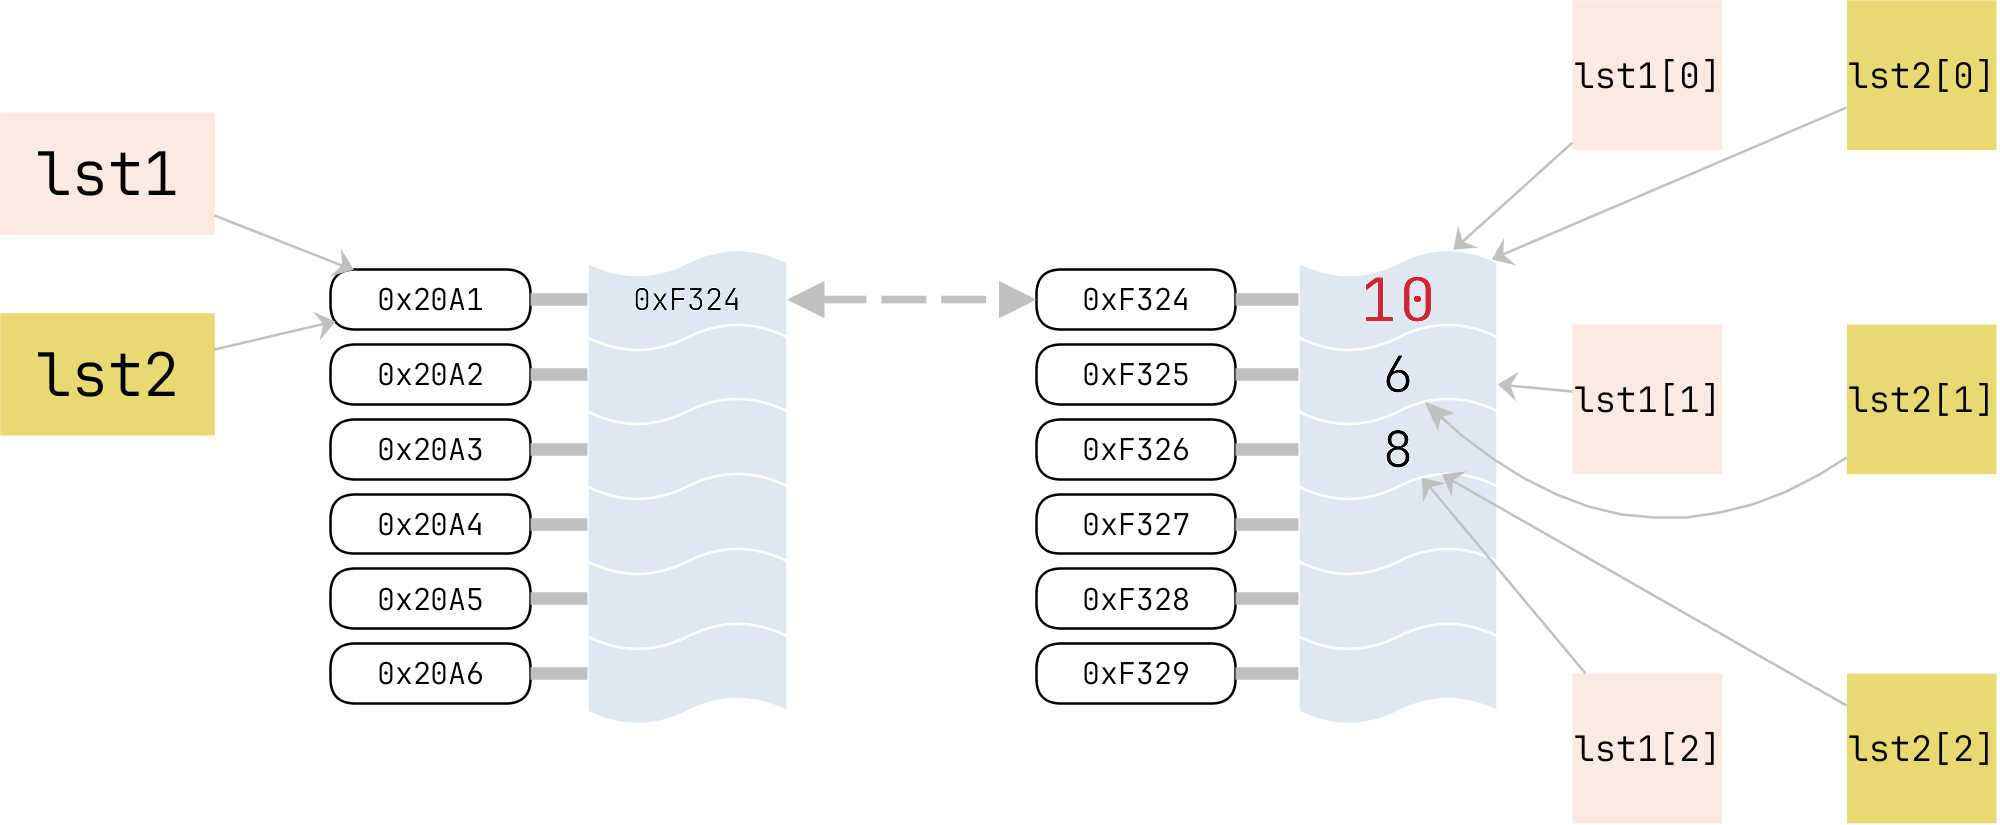
\includegraphics[width=\linewidth]{ch-listes/img/mut3.png} \\
Voilà donc pourquoi lorsqu'on écrit \mintinline{python}{lst2 = lst1}, tout changement dans \mintinline{python}{lst1} se reflète aussi dans \mintinline{python}{lst2} et vice-versa.\\

\subsubsection{Copier une liste (bonne méthode)}



\mintinline{python}{lst2 = lst1[:]}\\

Les éléments de \mintinline{python}{lst1} sont recopiés dans une autre zone mémoire, et \mintinline{python}{lst2} « pointe » sur l'adresse du début de cette zone.\\
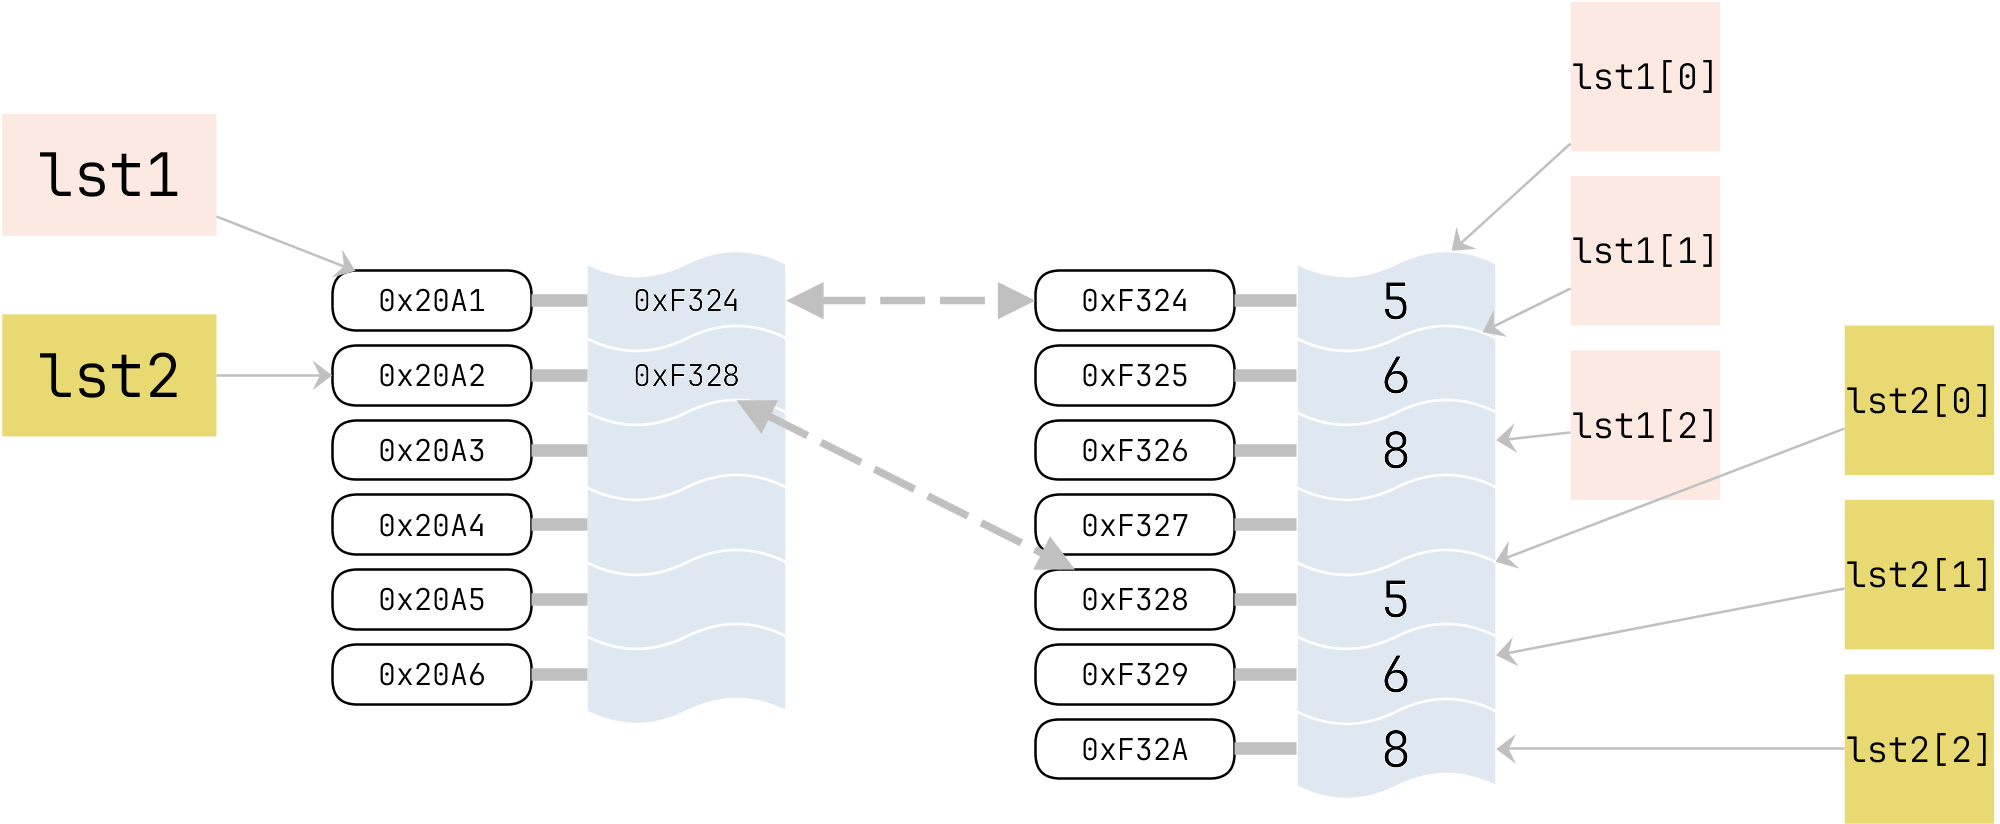
\includegraphics[width=\linewidth]{ch-listes/img/mut4.png}\\


\mintinline{python}{lst1[0] = 10}\\

Le changement n'affecte pas \mintinline{python}{lst2}.\\
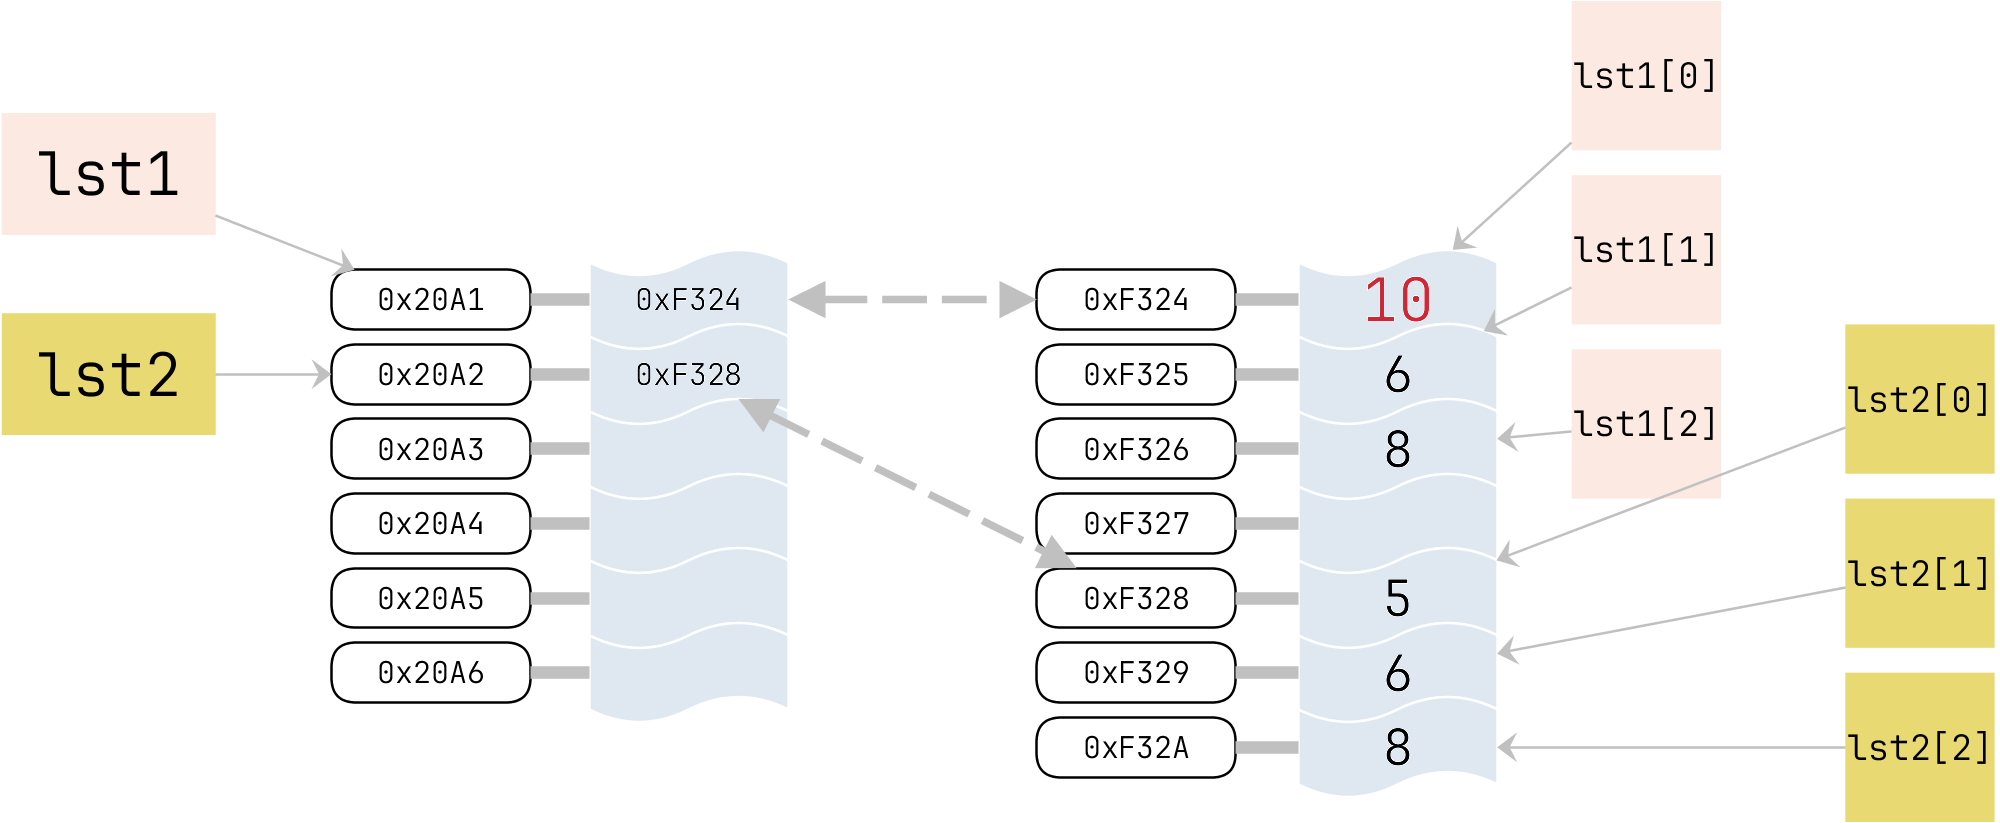
\includegraphics[width=\linewidth]{ch-listes/img/mut5.png}
% \chapter{Fonctions}
\introduction{Quelle est la fonction de ce chapitre ?}
\section{Exemples de fonctions}
\subsection{Un objet déjà connu}
Nous avons déjà rencontré des fonctions \textit{côté utilisateur}:
\begin{itemize}
    \item \mintinline{python}{input}
          \begin{itemize}
              \item prend en entrée une chaîne de caractères ;
              \item renvoie la chaîne de caractère saisie par l'utilisateur.
          \end{itemize}
          On peut noter ceci \mintinline{python}{input(chaine: str) -> str}
    \item \mintinline{python}{len}
          \begin{itemize}
              \item prend en entrée une liste ;
              \item renvoie le nombre d'éléments de cette liste.
          \end{itemize}
          On peut noter cela \mintinline{python}{len(lst: list) -> int}
\end{itemize}

\subsection{De multiples formes}
\floatpictureright{0.5}{ch-fonctions/img/fonction1}
{Les deux exemples précédents rentrent dans la catégorie représentée à droite.}
\medskip\par
\floatpictureleft{0.5}{ch-fonctions/img/fonction2}
{Certaines fonctions sont comme à gauche.\\
    Par exemple \mintinline{python}{max(20,3,10)} renvoie 20.}
\medskip\par
\floatpictureright{0.5}{ch-fonctions/img/fonction3}{
    D'autres fonctions sont comme à droite.\\
    On verra des exemples plus tard.}
\medskip\par
\floatpictureleft{0.5}{ch-fonctions/img/fonction4}{
    D'autres encore sont comme à gauche.\\
    Par exemple \mintinline{python}{print("salut")} ne renvoie rien mais affiche \mintinline{python}{salut} à l'écran.}
\medskip\par
\floatpictureright{0.5}{ch-fonctions/img/fonction5}{
    D'autres suivent le schéma ci-contre.\\
    Par exemple dans le module \mintinline{python}{time}, la fonction \mintinline{python}{time} ne prend aucun paramètre d'entrée mais renvoie l'heure qu'indique l'horloge de l'ordinateur.\\
    On peut par exemple l'utiliser pour stocker une heure précise en tapant \mintinline{python}{maintenant = time()}.}
\medskip\par
\floatpictureleft{0.5}{ch-fonctions/img/fonction6}{
    Enfin certaines suivent ce schéma.\\
    Par exemple dans le module \mintinline{python}{pygame}, \mintinline{python}{pygame.display.flip} ne prend aucun paramètre d'entrée, ne renvoie aucune valeur, mais actualise la fenêtre graphique.\\
    On l'appelle donc en tapant \mintinline{python}{pygame.display.flip()}.}
\medskip\par
Il est possible de créer de nouvelles fonctions.\\
On parle alors de fonctions \textit{côté concepteur}.\\

Il faut donc définir rigoureusement ce qu'est une fonction.

\section{Définition de la notion de fonction}
\begin{definition}[ : fonction]
    Une \textit{fonction} est un  «  morceau de code »  qui représente un \textit{sous-programme}.\\
    Elle a pour but d'effectuer une tâche \textit{de manière indépendante}.\\
\end{definition}

\begin{exemple}
    On veut modéliser la fonction mathématique $f$ définie pour tout nombre réel $x$ par $$f(x)=x^2+3x +2$$

    On écrira alors

    \begin{minted}[breaklines,breakanywhere]{python}
def f(x : float) -> float:
    return x ** 2 + 3 * x + 2
            \end{minted}

    Pour évaluer ce que vaut $f(10)$ et affecter cette valeur à une variable, on pourra désormais écrire \mintinline{python}{resultat = f(10)}.
\end{exemple}


Que fait la fonction \mintinline{python}{mystere} ?

\begin{minted}[breaklines,breakanywhere]{python}
def mystere(a : float, b : float) -> float:
    if a <= b:
        return b
    else:
        return a            
\end{minted}



La fonction \mintinline{python}{mystere}:
\begin{itemize}
    \item   prend en entrée deux paramètres de type \mintinline{python}{float} \mintinline{python}{a} et \mintinline{python}{b};
    \item   renvoie le plus grand de ces deux nombres.
\end{itemize}

La réponse que l'on vient de formuler s'appelle \textit{la spécification} de la fonction $f$.

\begin{definition}[ : fonction]
    Donner la spécification d'une fonction \mintinline{python}{f} c'est
    \begin{itemize}
        \item   préciser le(s) type(s) du (des) paramètre(s) d'entrée (s'il y en a) ;
        \item   indiquer sommairement ce que fait la fonction \mintinline{python}{f} ;
        \item   préciser le(s) type(s) de la (des) valeur(s) de sortie (s'il y en a).
    \end{itemize}
\end{definition}

\section{Anatomie d'une fonction}
\begin{pyc}
\begin{minted}{python}
def f(lst: list) -> int
    mini = lst[0]
    n = len(lst)
    for i in range(n):
        lst[i] < mini:
        mini = lst[i]
    return mini
   \end{minted}
\end{pyc}

La fonction \mintinline{python}{f}
\begin{itemize}
    \item   prend en entrée une liste (sous entendu d'entiers);
    \item   renvoie le plus petit entier de cette liste.
\end{itemize}

\subsection{Paramètre formel}

\floatpictureleft{0.5}{ch-fonctions/img/anat1}{
Le paramètre d'entrée est \textit{formel} : \textit{le nom de cette variable n'existe qu'à l'intérieur de la fonction}.
Si ce nom de variable existe déjà à l'extérieur de la fonction, \textit{ce n'est pas la même variable}.    
}\medskip\par

\floatpictureright{0.5}{ch-fonctions/img/anat4}{
Le type du paramètre d'entrée peut être spécifié. Ce n'est pas obligatoire mais très fortement recommandé pour  «  garder les idées claires » .
}\medskip\par

\subsection{Variables locales}
\floatpictureleft{0.5}{ch-fonctions/img/anat2}{
Toutes les variables \textit{créées} dans une fonction n'existent \textit{que dans cette fonction}. Elles ne sont pas accessibles depuis l'extérieur de la fonction. On dit que ce sont des \textit{variables locales}.}\medskip\par

\subsection{Valeur de sortie}
\floatpictureright{0.5}{ch-fonctions/img/anat3}{
Le type de la valeur de sortie peut être précisé, c'est également recommandé.    
}

\section{En pratique}
\subsection{Des exemples}
 \begin{pyc}
\begin{minted}{python}
1   def f(x : float) -> float:
2       return x ** 2 + 3 * x + 2
3    
4   print(f(1)) # Affiche 6
\end{minted}
\end{pyc}
Le programme commence à la ligne 4 !\\
Les 2 premières lignes servent à définir la fonction \texttt{f}, elles ne sont exécutées que lorsqu'on évalue \texttt{f(1)}.\\



\begin{pyc}
\begin{minted}{python}
def f(x : float) -> float:
    return x ** 2 + 3 * x + 2
    
print(x) # Provoque une erreur
\end{minted}
\end{pyc}
L'erreur vient du fait que la variable \texttt{x} \textit{n'est pas définie}. Le  «  \texttt{x} qu'on voit dans la fonction \texttt{f} »  est un paramètre formel et n'existe que dans \texttt{f}.\\


\begin{pyc}
\begin{minted}{python}
def f(x : float) -> float:
    a = 2
    return x + a

print(a) # Provoque une erreur
    \end{minted}
\end{pyc}
L'erreur vient du fait que la variable \texttt{a} \textit{est locale} : elle n'est définie que durant l'exécution de \texttt{f}.\\

\begin{pyc}
\begin{minted}{python}
def f(x : float) -> float:
    a = 2
    return x + a

print(f(4)) # Affiche 6        
print(a) # Provoque une erreur
    \end{minted}
\end{pyc}
C'est encore la même erreur : une fois \texttt{f(4)} évaluée, \texttt{a} n'existe plus.\\

\begin{pyc}
\begin{minted}{python}
1   def f(x : float) -> float:
2       a = 2
3       return x + a
4
5   a = 3
6   print(f(4)) # Affiche 6
7   print(a) # Affiche 3 et pas 2
\end{minted}
\end{pyc}

La variable \texttt{a} définie dans la fonction \texttt{f} n'est pas la même que celle qui est définie à la ligne 5.\\
Celle définie à la ligne 2 est \textit{locale}.\\
La variable \texttt{a} de la ligne 5 est appelée \textit{globale}.\\



\begin{pyc}
\begin{minted}{python}
def f(x : float) -> float:
    return x + a
        
a = 3
print(f(4)) # Affiche 7
\end{minted}
\end{pyc}
\begin{aretenir}
Une fonction a le droit d'\textit{accéder en lecture} à une variable globale, mais n'a pas \textit{a priori} le droit d'en modifier la valeur.
\end{aretenir}

\subsection{À éviter autant que possible}



\begin{pyc}
\begin{minted}{python}
1   def f(x : float) -> float:
2       global a 
3       a = a + 1
4       return x + a
5        
6   a = 3
7   print(f(4)) # Affiche 8
8   print(a) # Affiche 4       
\end{minted}
\end{pyc}
À la ligne 2, on signale à Python que \texttt{f} a la droit de modifier la variable globale \texttt{a}.
C'est fortement déconseillé : sauf si on ne peut pas faire autrement, une fonction ne doit pas modifier les variables globales.
% \chapter{\'Ecriture en compréhension}

\section{\'Ecritures simples}

Jusqu'à présent, pour construire des listes on a souvent :
\begin{itemize}
    \item    créé une liste \mintinline{python}{lst} vide ;
    \item    construit une boucle \mintinline{python}{for} ou \mintinline{python}{while} ;
    \item    peuplé la liste avec \mintinline{python}{lst.append}.
\end{itemize}

\begin{exemple}[]
    \begin{minted}{python}
        lst = []
        for i in range(10):
            lst.append(i*i)
        print(lst)
    \end{minted}
\end{exemple}


Ce programme affiche \mintinline{python}{[0, 1, 4, 9, 16, 25, 36, 49, 64, 81]}\\
C'est la liste des carrés des 10 premiers entiers naturels.\\
En mathématiques, l'ensemble des carrés des 10 premiers entiers naturels se note
\[\left\lbrace i^2\ |\ i\in\N,\,i<10\right\rbrace\]
C'est une écriture en \textit{compréhension}.\\
On peut faire la même chose en \textsc{Python} : \\

\mintinline{python}{lst = [i*i for i in range(10)]}\\

\'Evidemment, c'est plus rapide que la méthode précédente... Et on peut faire bien plus !
On peut utiliser une liste pour en construire une autre, par exemple en ajoutant 1 à chacun des éléments :
\begin{pyc}
    \begin{minted}{python}
    >>> lst1 = [2, -1, 3, 4, 7]
    >>> lst2 = [x + 1 for x in lst1]
    >>> lst2
    [3, 0, 4, 5, 8]
    \end{minted}
\end{pyc}
Dans le même esprit, on peut construire une liste dont les élements sont ceux de la première, mais avec une conversion de type :

\begin{pyc}
\begin{minted}{python}
>>> lst1 = ['2', '0', '13']
>>> lst2 = [int(x) for x in lst1]
>>> lst2
[2, 0, 13]
\end{minted}
\end{pyc}


Ou encore fabriquer la liste des initiales à partir d'une liste de prénoms :
\begin{pyc}
\begin{minted}{python}
>>> lst1 = ['Fred', 'Titouan', 'Tinaïg']
>>> lst2 = [prenom[0] for prenom in lst1]
>>> lst2
['F', 'T', 'T']
\end{minted}
\end{pyc}

\section{\'Ecritures avec conditions}



Il est possible d'utiliser \mintinline{python}{if} en compréhension : mettons dans \mintinline{python}{lst2} le double de chaque élément de \mintinline{python}{lst1} supérieur à 10 (dans l'ordre de parcours).
\begin{pyc}
\begin{minted}{python}
l>>> lst1 = [8, 0, 11, 10, 3, 15]
>>> lst2 = [2 * x for x in lst1 if x > 10]
>>> lst2
[22, 30]
\end{minted}
\end{pyc}



Il est possible d'utiliser \mintinline{python}{if ... else ...} en compréhension, mais à ce moment là il faut écrire les conditions au début   : créons une nouvelle liste en remplaçant tous les nombres négatifs de \mintinline{python}{lst1} par zéro.
\begin{pyc}
\begin{minted}{python}
>>> lst1 = [8, -10, 11, -4, -3, 15]
>>> lst2 = [(x if x > 0 else 0) for x in lst1]
# les parenthèses sont facultatives
>>> lst2
[8, 0, 11, 0, 0, 15]
\end{minted}
\end{pyc}

Créons une liste contenant les indices des éléments de \mintinline{python}{lst1} qui sont strictement positifs.
\begin{pyc}
\begin{minted}{python}
>>> lst1 = [8, -10, 11, -4, -3, 15]
>>> lst2 = [i for i in range(len(lst1)) if lst1[i] > 0]
>>> lst2
[0, 2, 5]
\end{minted}
\end{pyc}

\section{Les écritures en compréhension imbriquées}

$$\begin{matrix}
        0 & 0 & 0 & 0 \\0 & 0 & 0 & 0 \\0 & 0 & 0 & 0
    \end{matrix}$$
Si on veut représenter ce « tableau de nombres » par une liste, on peut écrire cet liste de 3 lignes comportant chacune 4 éléments :\\

\mintinline{python}{lst = [[0, 0, 0, 0], [0, 0, 0, 0], [0, 0, 0, 0]]}.\\

Cependant il est plus pratique d'écrire\\

\mintinline{python}{lst=[[0 for j in range(4)] for i in range(3)]}

\section{Pour conclure}

On peut combiner toutes les techniques que nous venons de voir. Par exemple on peut créer une liste de listes de listes avec des conditions, \textit{et c\ae tera}. La seule limite, c'est l'imagination et la capacité à écrire en \textsc{Python} !

% \chapter{Dictionnaires}
\section{Un nouveau type}

\picright{0.3}{ch-dictionnaires/img/dico}{
    On demande à des jeunes quel est leur sport préféré, les résultats sont présentés sur la figure ci-contre.\\
    Un sport peut être cité par \textit{plusieurs} jeunes, en revanche chaque jeune ne peut citer qu'\textit{un seul} sport.\\
    On pourrait utiliser une ou plusieurs listes pour représenter ces données mais il y a mieux : le \textit{dictionnaire}.
    La variable \mintinline{python}{sport} est de type \mintinline{python}{dict} :
}
\begin{pyc}
    \begin{minted}{python}
        sport = {'A': 'Tennis', 'B': 'Basket',
                 'C': 'Judo', ' D': 'Boxe',
                 'E': 'Foot', 'F': 'Gym',
                 'G': 'Foot'}
        \end{minted}
\end{pyc}


\begin{definition}[ : dictionnaire]
    Un dictionnaire est un ensemble d'\textit{éléments}.\\
    les éléments sont des couples de la forme \textit{clé : valeur}.\\

    La syntaxe est :\\ \mintinline{python}{variable = { cle1 : valeur1, cle2 : valeur2, ...}}\\

    Les valeurs peuvent être de n'importe quel type. Les clés peuvent être
    \begin{itemize}
        \item 	des \mintinline{python}{bool}, des \mintinline{python}{int}, des \mintinline{python}{float};
        \item 	des \mintinline{python}{str}...
        \item 	mais pas des \mintinline{python}{list} !
    \end{itemize}
\end{definition}


On peut tout de même utiliser des \mintinline{python}{tuples} en guise de clés :  les \mintinline{python}{tuples} ressemblent aux \mintinline{python}{list} mais sont \textit{non mutables}.\\

\mintinline{python}{a = (1, 2, 3)} est un exemple de \mintinline{python}{tuple}.

\section{Opérations sur les dictionnaires}

\subsection{Accéder à une valeur par sa clé}
Pour connaître le sport préféré de \mintinline{python}{'A'}, c'est simple :
\begin{pyc}
    \begin{minted}{python}
>>> sport['A']
'Tennis'        
    \end{minted}
\end{pyc}


\subsection{Créer de nouveaux couples clé: valeur}

Contrairement aux listes, il n'y a pas de méthode \texttt{append}.\\
Pour intégrer l'information « le sport préféré de H est le Rugby » on écrira simplement :\\
\begin{pyc}
    \begin{minted}{python}
        >>> sport['H']='Rugby'
    \end{minted}
\end{pyc}


\subsection{Créer un dictionnaire vide et le peupler}

On peut partir d'un dictionnaire vide et remplir ses valeurs au fur et à mesure :

\begin{pyc}
    \begin{minted}{python}
        >>> d = dict()
        >>> d['bonjour'] = 'hello'
        >>> d['crayon'] = 'pencil'
        >>> d['se prélasser'] = 'to bask'
    \end{minted}
\end{pyc}
\subsection{Supprimer un élément du dictionnaire}

\mintinline{python}{del d['crayon']} supprime l'élément \mintinline{python}{'crayon': 'pencil'}.

\subsection*{fusionner 2 dictionnaires}
\begin{minted}{python}
>>> d1 = {"anglais": "bread", 
          "français": "pain", 
          "slovaque": "chlieb"}
>>> d2 = {"allemand": "brot", "italien": "pane"}
>>> d1.update(d2) # fusionne d2 dans d1
>>> d1
{"anglais": "bread", "français": "pain", "slovaque": "chlieb", "allemand": "brot", "italien": "pane"}
\end{minted}

\subsection{Parcourir l'ensemble des clés d'un dictionnaire}
\begin{pyc}
    \begin{minted}{python}
    for cle in d1.keys():
        print(cle)
    \end{minted}
\end{pyc}
Ce script affiche
\begin{minted}{python}
anglais
français
slovaque
allemand
italien
\end{minted}

\subsection{Parcourir l'ensemble des valeurs d'un dictionnaire}
\begin{pyc}
    \begin{minted}{python}
for valeur in d1.values():
    print(valeur)
\end{minted}
\end{pyc}
Ce script affiche
\begin{minted}{python}
bread
pain
chlieb
brot
pane
\end{minted}

\subsection{Précisions}
\mintinline{python}{d1.keys()} et \mintinline{python}{d1.values()} ressemblent à des listes mais n'en sont pas !\footnote{Ce sont des \textit{itérateurs}, sctructures destinées à être parcourues. }\\

Pour avoir par exemple la liste des clés de \mintinline{python}{d1} on écrira :\\

\mintinline{python}{list(d1.keys())}\\

ou bien en \textit{compréhension} (ce qui revient au même mais peut s'avérer utile)

\mintinline{python}{[k for k in d1.keys()]}

\subsection{Erreurs de clé}
\begin{minted}{python}
print(d1['suédois'])
\end{minted}

Ce script produit une erreur :

{\color{red}\texttt{KeyError : 'suédois'}}

\begin{exemple}[ : Utilisation d'un dictionnaire]
    On veut créer un tableau de $10\times 10$ cases avec la valeur 0 dedans.\\

    On peut bien sûr créer cela avec une liste de listes (en compréhension) mais on peut également utiliser un dictionnaire :\\

    \mintinline{python}{{(x, y) : 0 for x in range(1, 11) for y in range(1, 11)}}\\

    \textbf{Avantages :}
    \begin{itemize}
        \item 	plus simple à manipuler : on écrit \mintinline{python}{d[x, y]} au lieu de \mintinline{python}{d[x][y]} ;
        \item 	on n'est pas obligé de faire commencer les indices à zéro.
    \end{itemize}

    \textbf{Inconvénients :}
    \begin{itemize}
        \item prend plus de place en mémoire (on s'en fiche un peu) ;
        \item plus flexible entraîne plus de possibilité d'erreurs !
    \end{itemize}
\end{exemple}


\section{Utilisation des dictionnaires}


Typiquement, pour stocker des \textit{données structurées} :    \\
\begin{minted}{python}
reseau = {'nom'        : 'local',
          'ip'         : '192.168.1.0',
          'masque'     : '255.255.255.0',
          'passerelle' : '192.168.1.254'}
\end{minted}

On utilise fréquemment des listes de dictionnaires, ou bien des dictionnaires de listes.

% \tableofcontents
\end{document}